% !TEX program = pdflatex+makeindex+bibtex
% !TEX encoding = UTF-8 Unicodede_ch

% created by Simon Schälli <simon.schaelli@kantiwattwil.ch>
% v1.0 ursprüngliche Version
% v1.1 2015-10-22 mit Titelbild
% v1.2 2016-09-30 aufgeräumt
% v1.3 2016-10-16 Layoutfehler behoben

%======================================================================%
%=== Dokument auf häufige Fehler überprüfen                         ===%
%======================================================================%
\RequirePackage[l2tabu, orthodox]{nag}

%======================================================================%
%=== Dokumentklasse wählen                                          ===%
%======================================================================%
\documentclass[a4paper,openright,12pt]{scrreprt}

%======================================================================%
%=== Pakete einbinden                                               ===%
%======================================================================%
\usepackage[utf8]{inputenc}
\usepackage[english]{babel}


% Latin Modern Schriftart
\usepackage{lmodern}
\usepackage[T1]{fontenc}


% Mathematik-Pakete
\usepackage{amsmath}
\usepackage{amssymb}
\usepackage[mathscr]{euscript}
\usepackage{mathtools}

% mathematische Buchstaben als Text
\usepackage{textcomp}

% komfortable Referenzen mit \fref
\usepackage[english]{fancyref}

% Kopf- und Fusszeilen
\usepackage[automark,headsepline]{scrpage2}
\ihead[]{\headmark}
\chead[]{}
\ohead[]{\pagemark}
\ifoot[]{}
\cfoot[\pagemark]{}
\ofoot[]{}
\pagestyle{scrheadings}

% Einfügen von Bildern¨
\usepackage{float}
\usepackage{graphicx}
\usepackage{subfig}

% schöne Tabellen
\usepackage{booktabs}
\captionsetup[table]{font=small,skip=0pt}

% Tabelleninhalt an Dezimalpunkt ausrichten
\usepackage{dcolumn}
\makeatletter                     % <- hebt Sonderbedeutung von @ auf
\newcolumntype{d}[1]{D{.}{.}{#1}} % <- definiert einen neuen Spaltentyp
\makeatother                      % <- setzt Sonderbedeutung von @ wieder

% Algorithms
\usepackage[ruled,vlined]{algorithm2e}
\SetKwInput{KwRequire}{Require}

% code
\usepackage{xcolor}
\definecolor{bluekeywords}{rgb}{0.13,0.13,1}
\definecolor{greencomments}{rgb}{0,0.5,0}
\definecolor{redstrings}{rgb}{0.9,0,0}
\definecolor{codegreen}{rgb}{0,0.6,0}
\definecolor{codegray}{rgb}{0.5,0.5,0.5}
\definecolor{codepurple}{rgb}{0.5,0,1.0}

\usepackage{listings}
\lstset{language=Python,
showspaces=false,
showtabs=false,
breaklines=true,
showstringspaces=false,
breakatwhitespace=true,
escapeinside={(*@}{@*)},
keywordstyle=\color{bluekeywords}\bfseries,
stringstyle=\color{redstrings},
basicstyle=\ttfamily
}

%Color Boxes, proofs
\usepackage{tikz,lipsum,lmodern}
\usepackage[most]{tcolorbox}

% Beispieltext
\usepackage{lipsum}

% Hyperlinks in PDF
\usepackage{hyperref}

% Biblatex
\usepackage[
backend=biber,
style=numeric,
sorting=ynt
]{biblatex}
\addbibresource{mybib.bib}

% Macros
\usepackage{mymacros}
\usepackage{xargs}

%======================================================================%
%=== Angaben zum Dokument                                           ===%
%======================================================================%

\titlehead{Kantonsschule im Lee \hfill Kalani Fin Kistler\\
Fachschaft Mathematik \hfill Dättnauerstrasse 107\\
% Rychenbergstrasse \hfill 8406 Winterthur\\
% 8400 Winterthur
}
\subject{Matura Thesis 20/21}
\title{Policy Gradient Based Reinforcement Learning Applied to Playing Soccer}
\author{\texorpdfstring{Kalani Fin Kistler, 4h \\[1cm]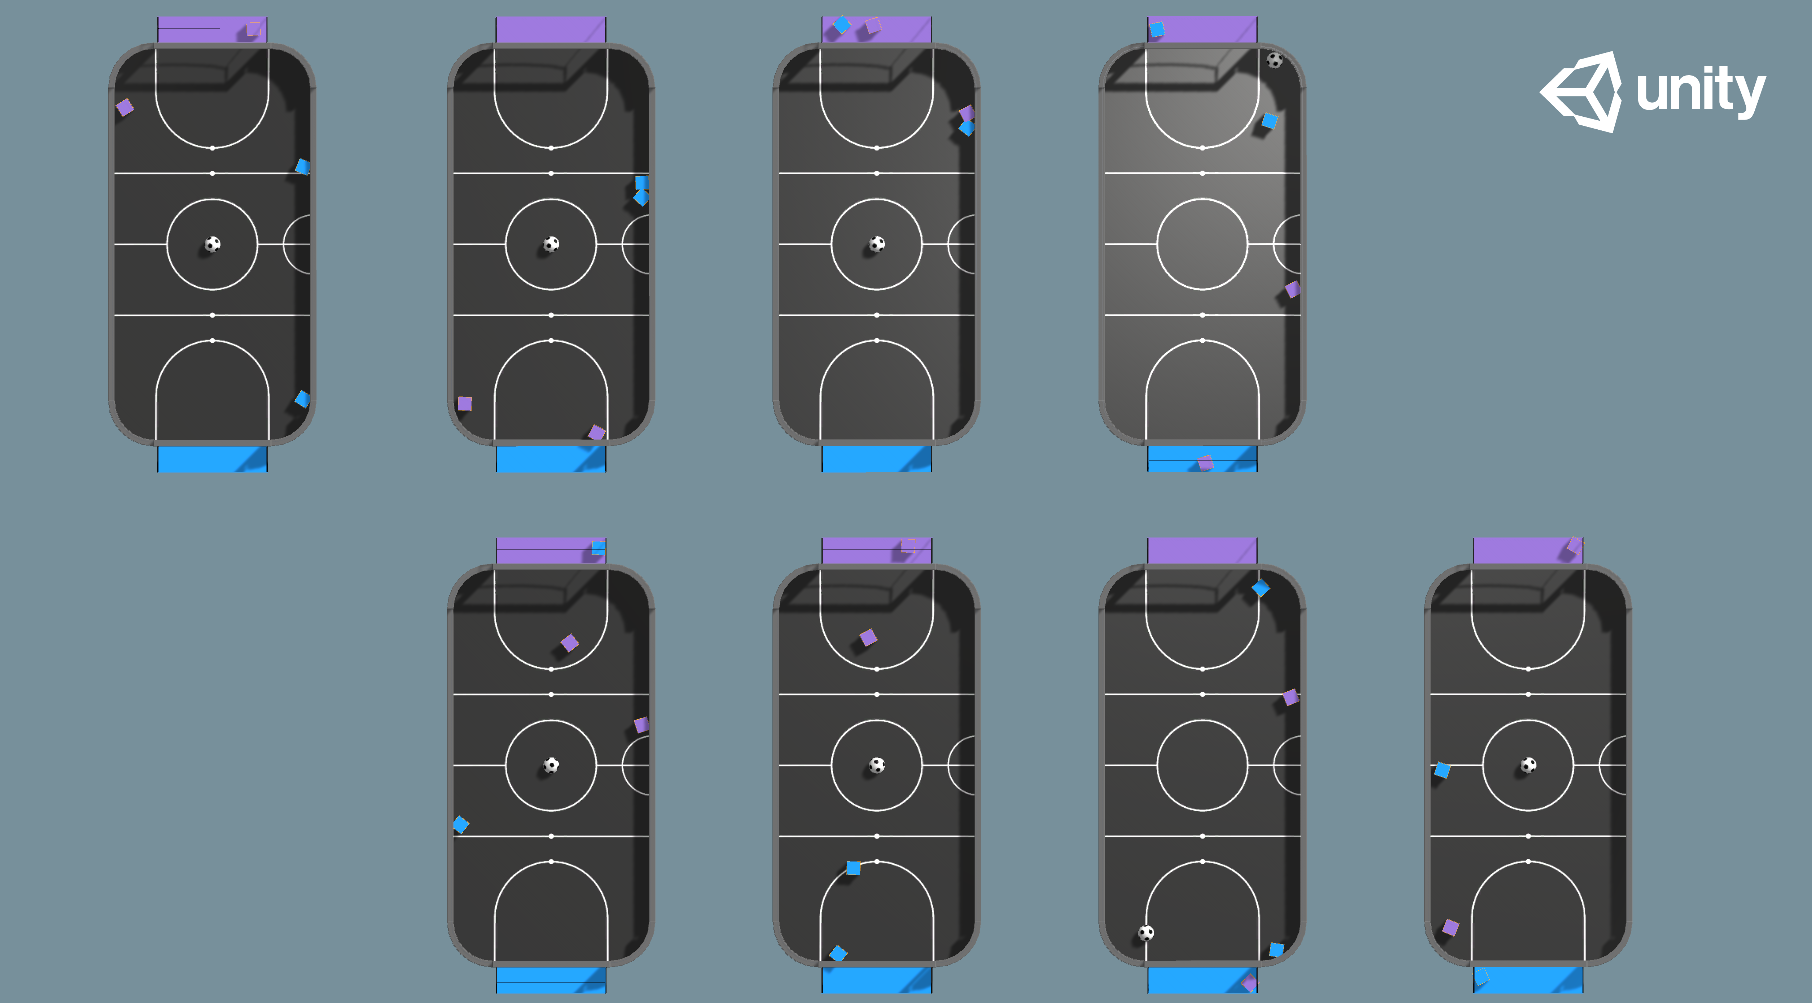
\includegraphics[scale=0.2]{figures/Screenshot from 2020-09-22 23-05-59.png}\\[1cm] {\small Supervisor: Elena Fattorini}}{Kalani Fin Kistler 4h}}
\date{\small Winterthur, 04.01.2021}
%======================================================================%
%=== PDF Dokumenteinstellungen                                      ===%
%======================================================================%

\makeatletter
\hypersetup{
	pdftitle={\@title},%
	pdfsubject={\@subject},%
	pdfauthor={\@author},%
	pdfkeywords={},%
	colorlinks,%
	citecolor=black,%
	filecolor=black,%
	linkcolor=black,%
	urlcolor=black}
\makeatother

\linespread{1}

\usepackage{geometry}
 \geometry{
 a4paper,
 right=30mm,
 left=30mm,
 top=30mm,
 }

%======================================================================%
%=== Beginn des eigentlichen Dokumentes                             ===%
%======================================================================%

\begin{document}

\fontfamily{lmr}\selectfont

\maketitle % <- Titel setzen
\cleardoublepage
\pagenumbering{roman} % <- römische Seitennummerierung
\tableofcontents % <- Inhaltsverzeichnis
\cleardoublepage % <- neue Seite
\pagenumbering{arabic} % <- arabische Seitennummerierung


% !TEX root = ../maturaarbeit.tex
\chapter{Introduction}\label{chap:einleitung}

% !TEX root = ../maturaarbeit.tex
\chapter{Background}\label{chap:background}
% !TEX root = ../maturaarbeit.tex
\section{What is Reinforcement Learning?}\label{sec:what_is_rl}
\noindent
Throughout our daily lives we navigate our surroundings, handle social situations and tackle complex tasks. In doing, so we take the actions we believe, based on experience and intuition, to have the best outcome. We might take these abilities for granted, given how natural they are to us. However, at some point we had to obtain these skills so essential in managing our day to day, many through simple trial and error. Reinforcement Learning (RL) seeks to formalize the process of figuring out how to behave based on what produces desirable results and what does not, and adjusting our future actions accordingly. 

\noindent
\\ Reinforcement Learning is a discipline of machine learning \cite[p. 1]{sutton_reinforcement_2018}, an incredibly broad field which is focused on the optimization of computer algorithms by processing data and experience. As such it is an intersection between the natural, to us intuitive concept of learning, and the rigid and numerical world of computer programming and mathematics \cite[p. 4]{sutton_reinforcement_2018}. To be able to understand how this learning process works, and to be able to quantify and formalize it, it is essential to introduce some general concepts. 

\subsection{Illustrative Example: Card game UNO}\label{subsec:UNO}

\begin{figure}[ht]
    \centering
    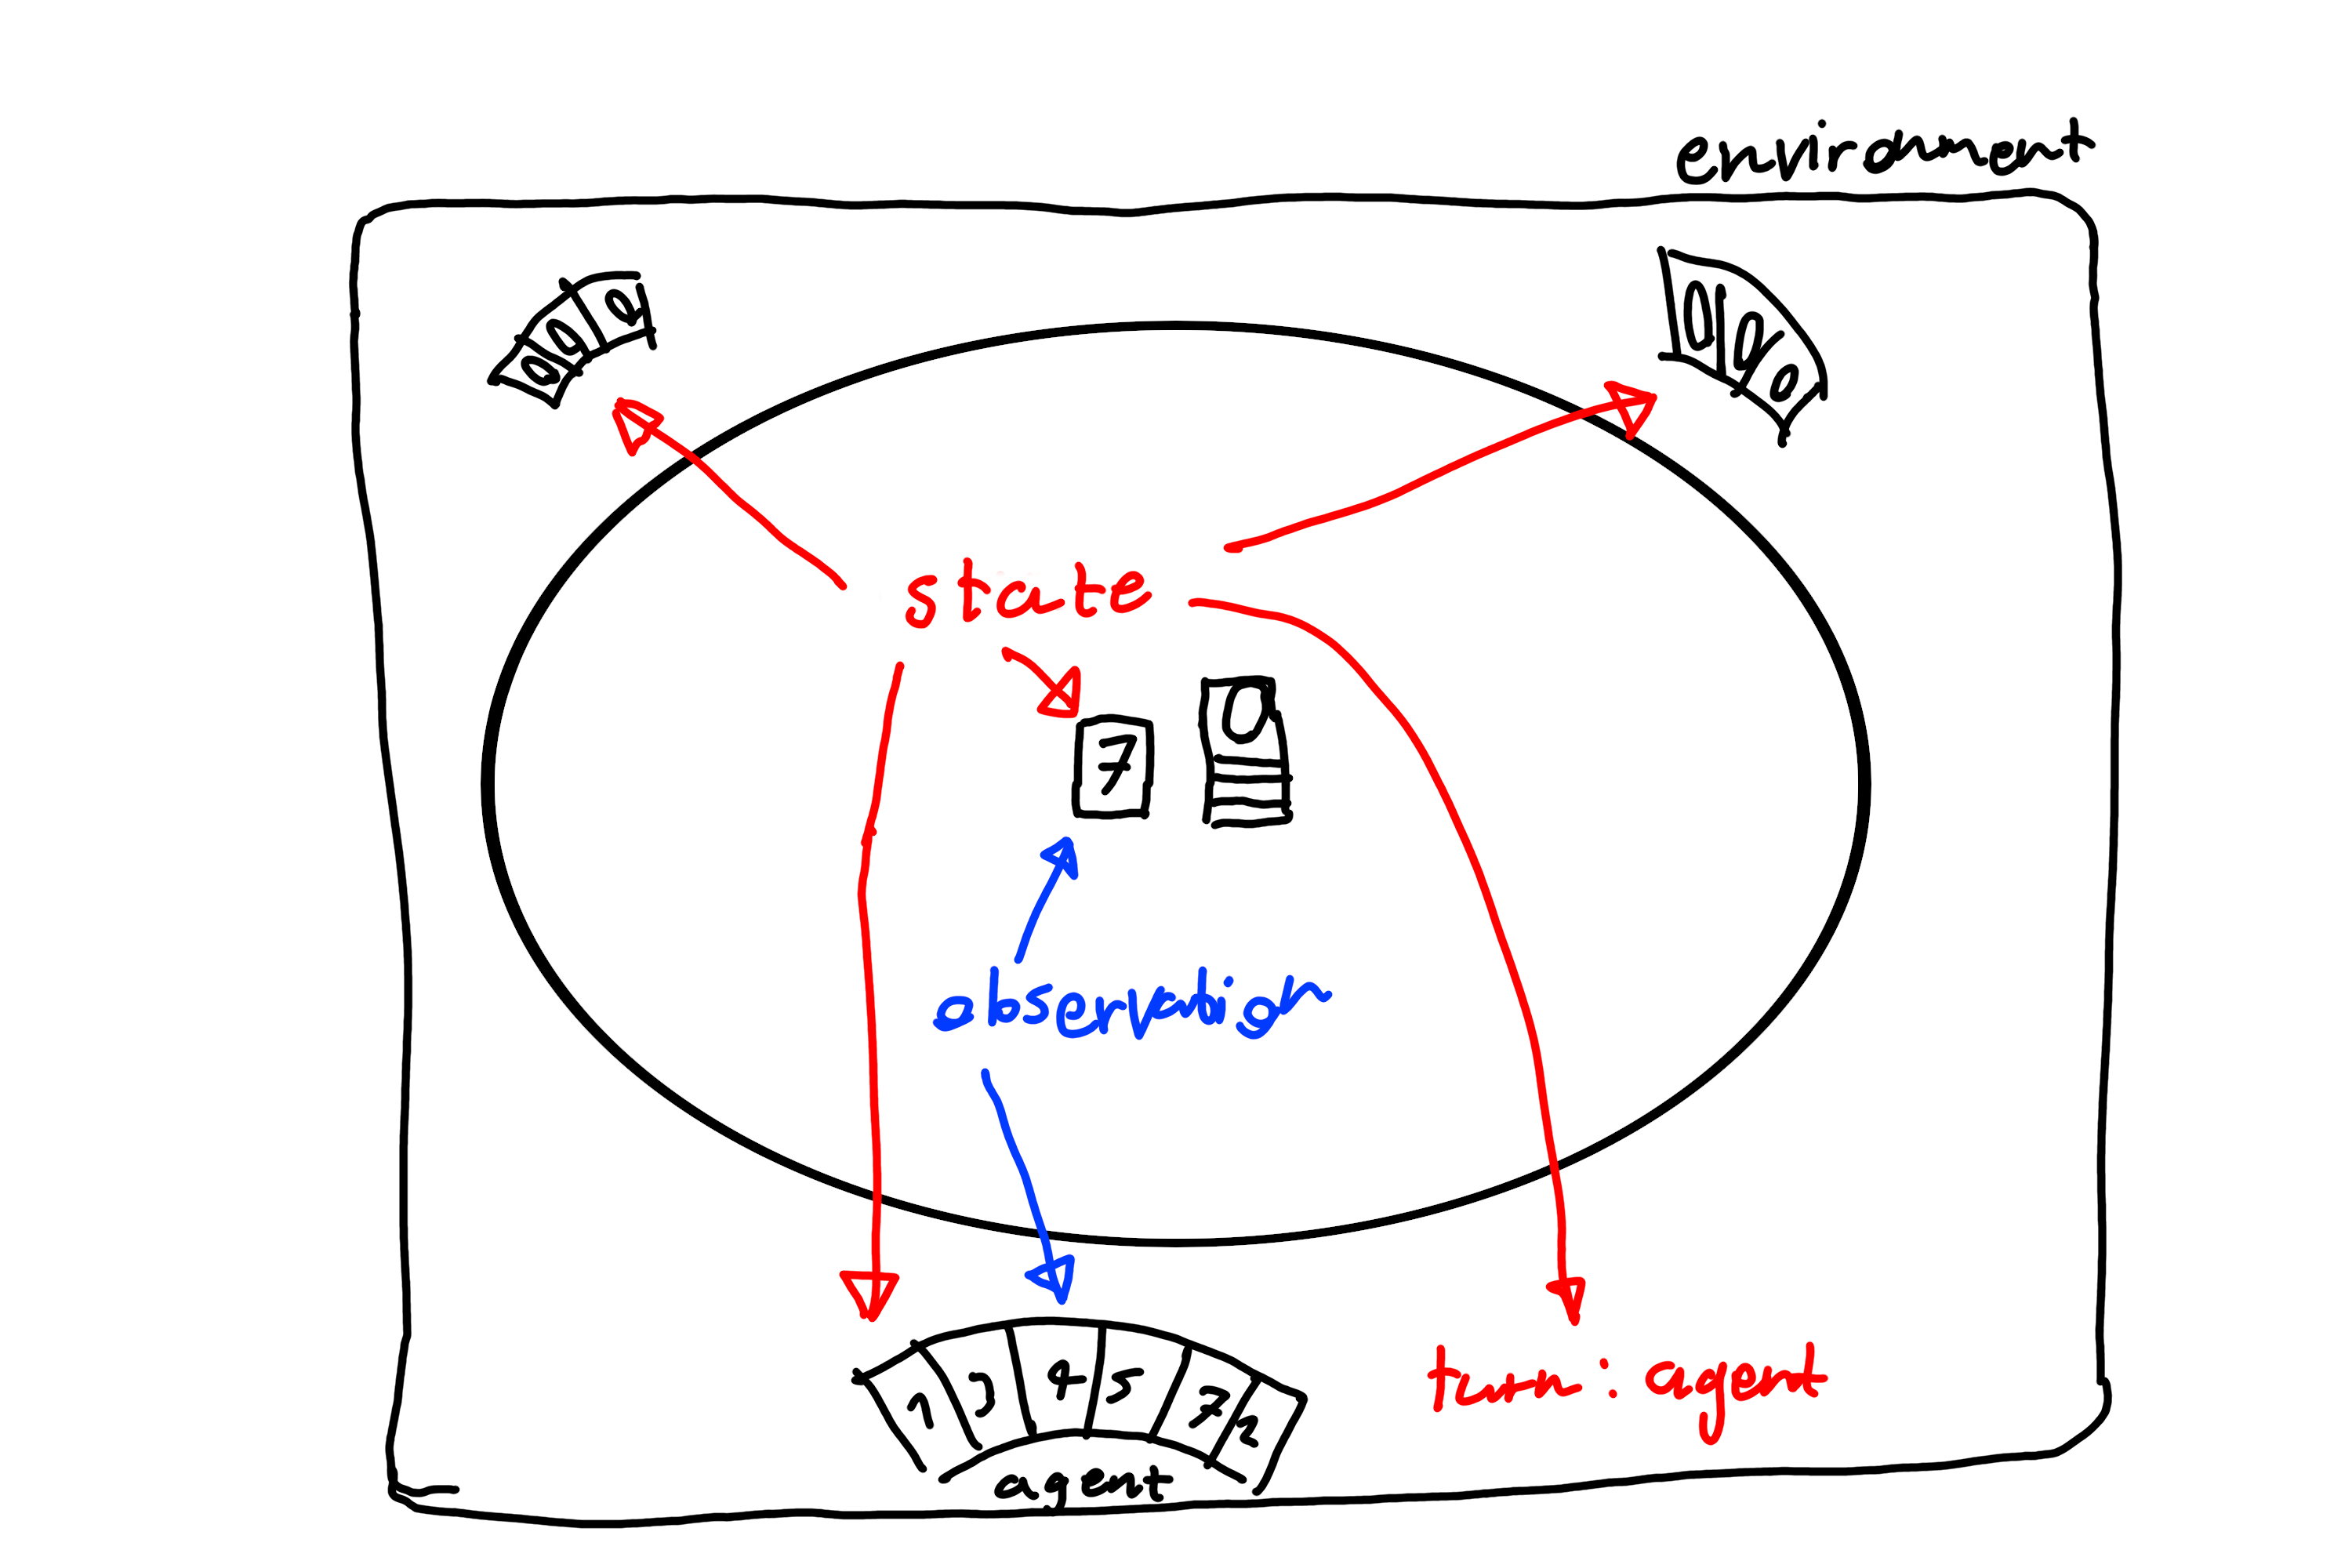
\includegraphics[width=\linewidth]{figures/UNO.png}
    \caption{UNO environment in the context of RL}
    \label{fig:UNO}
\end{figure}

\noindent
Consider the example of teaching someone how to play the popular card game “UNO”. The \textit{objective} of the game is to get rid of the cards on your hand before the other players. We can call the game an \textit{environment}. This environment contains all the players players, including their strategies, the cards and what rules the game follows. A state of an environment describes the arrangement of all components encompassed by it, in this case the hands of the players, who's turn it is, what cards are on which pile and their order. Notice that the environment contains a lot of information which the player, in Reinforcement Learning called an \textit{agent} (an actor in the environment) does not know. However, the actor can \textit{observe} the environment and thereby gain a reasonably accurate representation of it’s state. Suppose it is the agent's turn. Based on its \textit{observation} the agent can take an \textit{action a}, playing any of the cards on its hand, or picking one up. The rules of an environment might forbid certain actions, taking one of them, will lead to the same environment state, where it is the agents turn. A well designed environment will give the agent negative feedback, when teaching someone UNO, that might be telling them they did something wrong. In Reinforcement Learning this is called \textit{reward signal}. Based on the \textit{reward}, the agent then can update its behaviour to produce a different action next time. Thereby the reward \textit{reinforces} the desired behaviour, it is a \textit{reinforcement} the agent learns from. The way of acting of an agent in a state given, an observation of that state, is called a \textit{policy}, commonly denoted as $\pi$. The agent follows a policy to decide on an action, based on a state.
\newline
For the sake of brevity, unless the distinction is relevant, I am going to use the terms observation and state interchangeably. Much more expansive definitions going in to the nuances of these concepts can be found in the book \textit{Reinforcement Learning, An introduction} by Richard Sutton and Andrew Barto. \cite{sutton_reinforcement_2018}

\subsection{What Type of Problem does Reinforcement Learning suit?}\label{subsec:Why_RL}
When solving a problem where the environments rules are well known like UNO Reinforcement Learning might indeed not be the best approach. In the case of UNO, it might be more efficient to design an algorithm which computes some probability of victory for each action, based on what cards have been played and then picks the optimal one. However, this approach requires knowledge of how the environment operates \cite[p. 8]{sutton_reinforcement_2018}, if for example, it was not know what happens after our turn, it would suddenly become nigh impossible to explicitly define a probability of victory for an action. Another issue that quickly arises as the environment becomes more complex, is the rapid rise in the number of its possible permutations. Accounting for all of them quickly becomes unfeasible as the environment grows more complex. Reinforcement Learning lets us generate high quality solutions in uncertain environments based on a reward signal and the goal it ultimately describes \cite[p. 03]{sutton_reinforcement_2018}. Another approach which might come to mind as an obvious solution would be to simply mimic the behaviour of an optimal, or close to optimal, agent. However, this again is impractical as such an agent might simply not exist or generating sufficient examples can be tedious. As stated in Reinforcement Learning, An Introduction: “In uncharted territory—where one would expect learning to be most beneficial, an agent must be able to learn from its own experience.” \cite[p. 02]{sutton_reinforcement_2018} Here it is important to keep in mind that machines see environments differently from humans. For a human the actions involved in pouring a coffee, might be to pick up the can and tilt it. Plenty of examples exist on how to do that. However, we are only able to make sense of the example because we intuitively understand how move our limbs, the instructions of "pick up and tilt" would be useless to a robot which views the world through a grid of pixels and which can take only take actions in the form of powering a series of motors which move an arm, it would need an example which matches its way of interaction with the environment.

\section{The Finite Markov Decision Processes, a mathematical framework for Reinforcement Learning}\label{sec:MDP} % NOTE: THESE ARE ALL REFERENCES TO THE BOOK
I this section I will introduce Finite Markov Decision Processes (MDPs) which serve as a formalization of sequential decision making. Problems which can be described as a finite MDP are what Reinforcement Learning is trying to solve. They are called finite because the sets $\mathset{S}, \mathset{A}, \mathset{R}$ of all states, actions, and rewards respectively, are all finite. I will illustrate and apply the concepts in this section using a Grid-World environment. It serves as a particularly convenient example since in it, the state of the environment is fully described by the agent's position. This allows for simple computation and visualization. 

\subsection{Sequential decision making}\label{subsec:sequential_decision_making}
In an MDP the agent and environment continually interact. At each time step $t$ of that interaction, the agent selects an action, the environment transitions in to a new state $S_{t+1}$ and gives the reward $R_{t+1}$. Based on this new state, the agent selects another action. This series of interactions may go on forever. From this there also follows that states can be revisited, a finite set of states could not support an infinite series of transitions otherwise. $S_ {t+1}$ is just the state which the environment transitions to next and does not refer to a specific state in the set of states, the environment may even transition back to itself, in that case $S_t$ and $S_{t+1}$ would be identical. This is possible because all possible futures solely depend on that state, else it would not fully describe the environment.

\begin{figure}[h!]
    \centering
    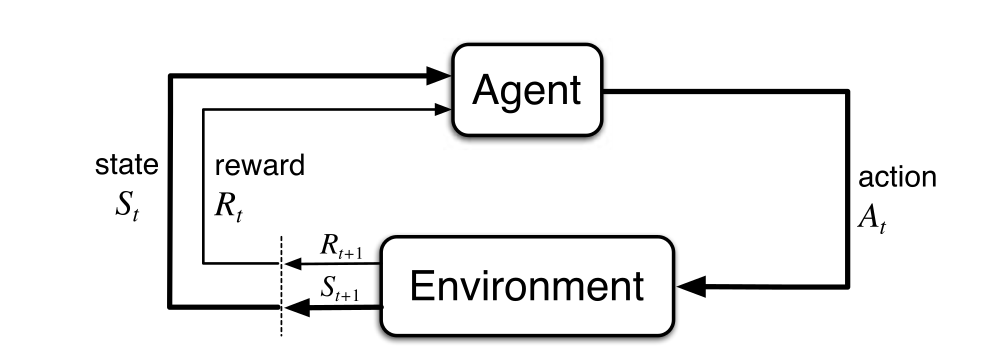
\includegraphics[width=0.7\linewidth]{figures/agent_environment_interaction_loop.png}
    \caption{Agent Environment Interaction Loop as presented in \citepg{48}}
    \label{fig:agent_env_inter}
\end{figure}

\noindent
Since the agent environment interaction is sequential, a sequence, or in Reinforcement Learning \textit{trajectory} $\tau$, arises. \citepg{48}

\begin{equation}\label{MDP:trajectory}
    \Tau = S_0, A_0, R_1, S_1, A_1, R_2 \dots
\end{equation}
\centerline{\small\textit{from \citepg{48}}}

\noindent
\\ In an \ita{episodic} environment, an environment that ends at some terminal time-step $T$, a trajectory has a terminal state $S_T$ and reward $R_T$. The notion of a terminal action does not make sense since the environment terminates at $T$, any action taken would not have an effect, and the action which proceeds $S_T$ is $A_{T-1}$.

\subsubsection{Illustrating in Grid-World}\label{subsubsec:grid_world_trajectory}
The Agent starts at a starting position, here the bottom left corner, and has to reach the upper right corner, by choosing from the actions up, down, left, right at each time step. The blacked out fields are inaccessible, running in to them or the walls, just results in the same state, the agent does not move. The rewards are not yet displayed here to avoid clutter, they will be discussed in the next section.

\begin{figure}[h!]
    \centering
    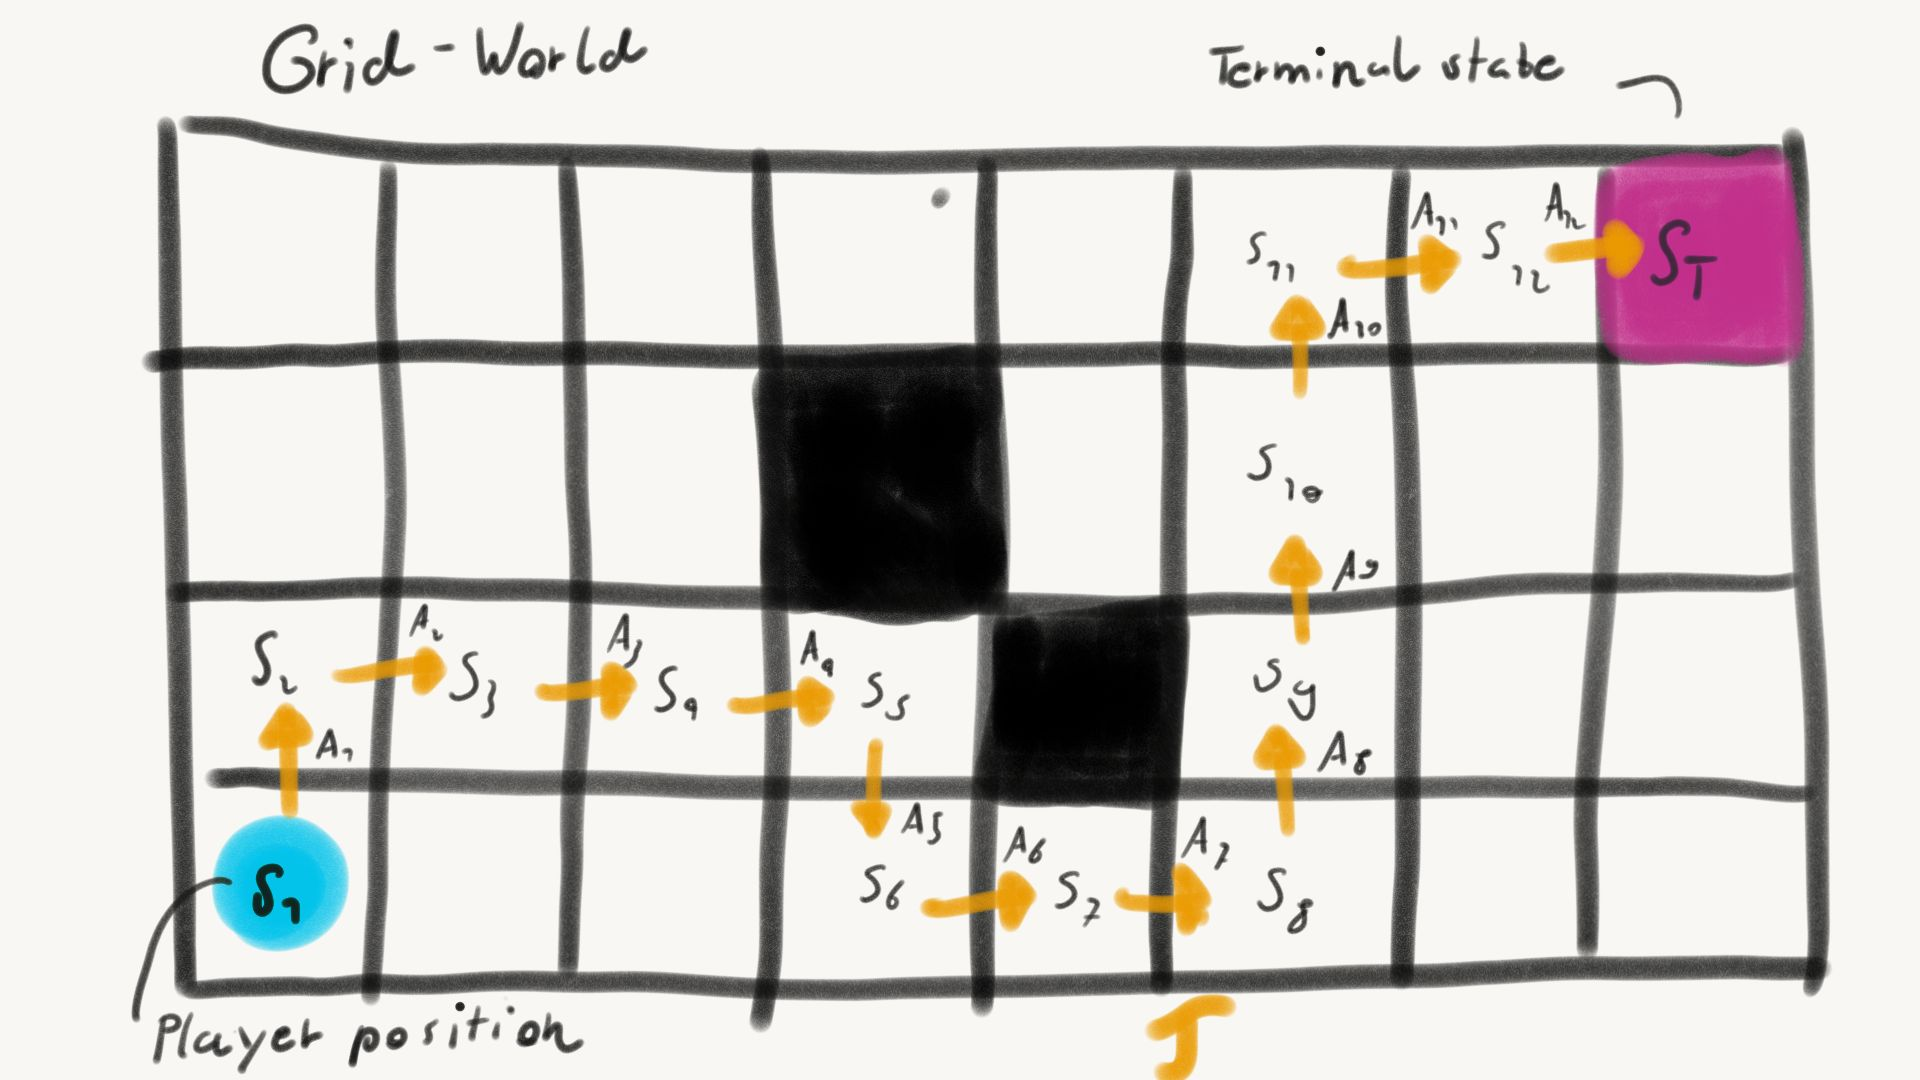
\includegraphics[width=0.7\linewidth]{figures/Grid_world_trajectory.jpeg}
    \caption{The Grid World Environment}
    \label{fig:grid_world}
\end{figure}

\noindent
The agent then moves through the states and therein generates a trajectory. The representation of that trajectory overlaid on to the grid, works in this case because the agents position fully describes an environment state. Archiving an agents trajectory becomes useful when evaluating and training the agent, since an evaluation based upon a series of correlated events, is obviously more meaningful, than one based entirely on one singular action and its consequence.

\subsection{Agent Policies in a MDP}\label{subsec:policies}

Moving forward it is important to understand what policies are mathematically. So far it has been established that policies are the way in which an chooses an action based on a state. Policies do not have to be deterministic. Mathematically, the policy is a function which takes a state and produces a probability distribution over the set of actions. This function can be parameterized, the parameter vecotr is commonly written as $\theta$. This distribution can be discrete or continuous and may produce vector actions. An action can be obtained from a policy by sampling from it. This is outlined in \citepg{58}, where $\pi(a|s)$ is defined as the probability of $a$ given $s$ under $\pi$. In our example of grid world the policy would be a discrete distribution. If the policy is parameterized, then $\pi(a|s)$ becomes $\pi(a|s,\theta)$. 

\subsection{The episodes Return, an improved measure of agent performance}\label{subsec:goals}

The agent selects actions based on state information and and receives rewards as feedback for its previous action. The goal of the agent is to maximize the reward signal received. It does that by updating its policy to produce a better action $A_t$ in the state $S_t$ based on the signal received at $t$. This means that one of the ways in which we can improve learning performance is to tweak the reward signal. The perhaps most obvious signal to give the agent is the reward $R_{t+1}$ which followed its action. However this does not take in to account any of the future states and rewards the agent's action lead to, it would not at all plan for any future states and rewards. To curb this issue we introduce the \textit{return} $G_t$. In contrast to the reward, the return also considers the influence of $A_t$ on future rewards. It is defined as follows:

\begin{equation}\label{MDP:return}
    G_t \doteq R_t + R_{t+1} + R_{t+2} \dots + R_T
\end{equation}
\centerline{\small{\ita{\citepg{54}}}}

\noindent
\\ Although the return undoubtedly is a better measure of the "goodness" of an action than the reward and training the agent using it produces decent results, it still has some flaws. Of these the most relevant to my work is that taking the sum of the rewards from the current time step to the episode's end gives the same weight to all the rewards. In many environments $A_{t-600}$ is much less relevant to $R_{t+1}$ then $A_t$, yet $R_{t+1}$ has the same weight in $G_{t}$ as it has in $G_{t-600}$. To address this, the discounted return can be used. 

\begin{equation}\label{MDP:discounted_return}
    G_t = \sum_{k=t}^{T} R_{t+k+1} \cdot \gamma ^k 
\end{equation}
or recursively as
\begin{equation}\label{MDP:recursive_discounted_return}
    R_{t+1} + \gamma \cdot G_{t+2} \mathrm{\ where\ } 0 \leq \gamma \leq 1
\end{equation}
\centerline{\small{\ita{\citepg{55}}}}

\noindent
\\ By tweaking the discount factor we can balance immediate reward with future ones. It is another hyper parameter that needs to be set which affects agent performance. Discounting also enables the use of the return in continuous environments, it is why it was originally introduced and is the main reason it is presented in \cite{sutton_reinforcement_2018}. {\\ \color{red} SHOW RESULTS OF DISCOUNT FACTOR 1 VS 0.99 AND SAY THAT IT IS BAD} \\ The returns in Grid-World with different discount factors can be seen here:

\begin{figure}[h!]
    \centering
    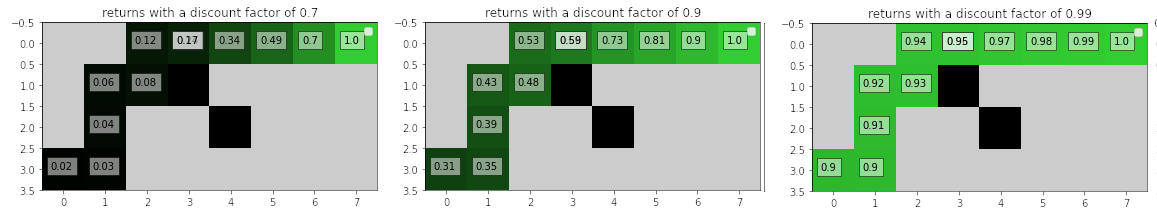
\includegraphics[width=\linewidth]{figures/grid_world_discount_factors.png}
    \caption{Returns for each time step in an episode for different discount factors}
    \label{fig:grid_world_discount_factors}
\end{figure}

\noindent
\\ The only reward the agent receives here occurs on the final time-step, and has a magnitude of 1. Notice how quickly the return decays with even a discount factor 0.9. This makes the agent quite short sighted. Due to its exponential decay small discount factors often do not make sense.

\noindent
\\ Optimizing for the return is still dependant on the quality of the rewards. Ideally, rewards should represent the thing we want the agent to achieve. Since they are the only information the agent can learn from should also not be too sparse. The problem of dealing with environments which give sparse reward is a large hurdle in modern day RL, some solutions to this are addressed in \citepg{491}. In such environments it turns out to be useful to modify the rewards received by setting baselines, creating "intrinsic rewards", those could for example be rewards for exploring the environment and many others. 

\subsection{Simple Solution for Grid-World using the presented concepts}
TODO



\section{Optimization with Gradient Descent}\label{gd}
All throughout Machine Learning gradient descent and variations of it are used for optimization. Gradient descent is vital for my work. As such I will briefly explain what it is and how it is relevant to my work.

\subsection{What is Gradient Descent?}\label{gd:what_is_it}
In essence gradient descent is an algorithm used to find local minima of differentiable functions. It can be thought of as starting at a point on the function graph and walking down hill until one reaches a minimum. Gradient descent works by differentiating a function at some point in order to obtain a slope, and then moving in the downwards direction of that slope. Gradient descent is done in steps. If $f(\theta)$ is a differentiable function, then one gradient descent step is:

\begin{equation}\label{Graident_Descent:basic_update}
    \theta \leftarrow \theta - \alpha \cdot \frac{\partial}{\partial \theta}f(\theta)
\end{equation}

\noindent
\\ The \textit{step size} $\alpha$ is introduced to control the magnitude of the descent step. The gradient descent algorithm consists of performing these steps iteratively until the current value (in the above case $\theta$) is sufficiently close to the actual local minimum. Performing 10 gradient descent steps on the function $f(\theta) = \theta^2$ and a starting value of $\theta = 3$ with various values for alpha looks as follows:

\begin{figure}[ht]
    \centering
    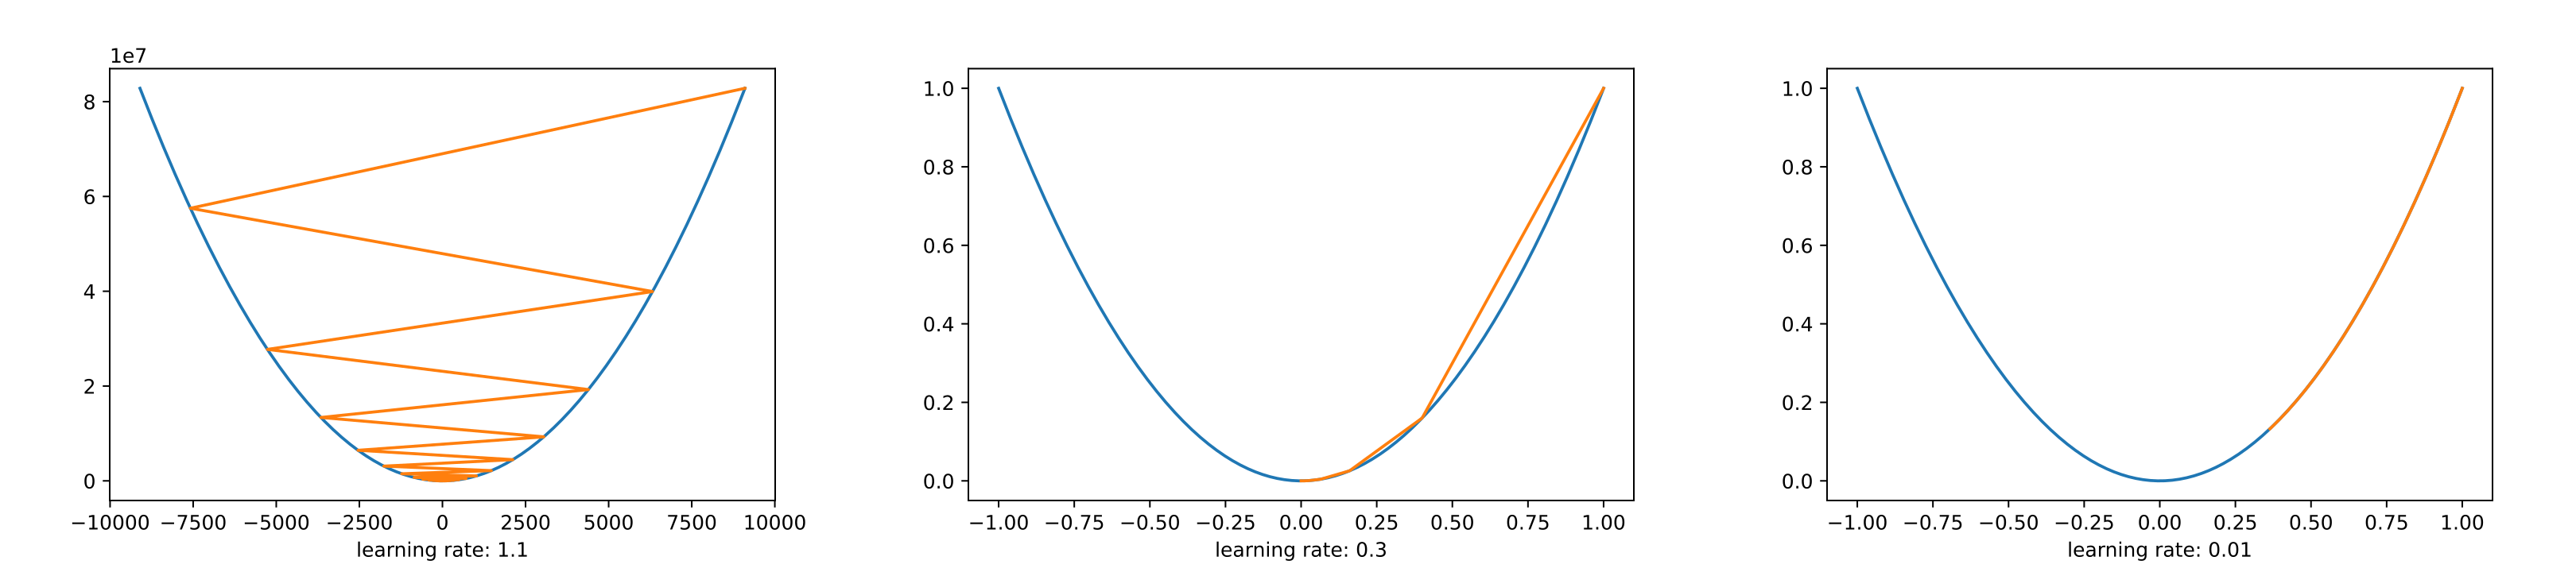
\includegraphics[width=\linewidth]{figures/grad_desc.png}
    \caption{Gradient Descent on $f(\theta) = \theta^2$}
    \label{fig:UNO}
\end{figure}

\noindent
\\ As can be clearly seen here smaller step sizes lead to more accurate results. Too large a step size may even lead to divergence. However, if the step size is too small, it may take very long to reach a local minimum. Gradient descent functions in the exact same way if $\theta$ is a vector. In that case the update step becomes:

\begin{equation}\label{Graident_Descent:basic_update_vector}
    \theta \leftarrow \theta - \alpha \cdot \nabla_\theta f(\theta)
\end{equation}

\subsubsection{Gradient Ascent}\label{gd:gradient_ascent}
As the name implies gradient ascent is the exact opposite of gradient descent. Instead of trying to find the local minimum of a function, when performing gradient ascent we are trying to find the local maximum of a function. Gradient Ascent is identical to performing Gradient Descent on the negative derivatives. 

\subsection{How is Gradient Descent relevant to Reinforcement Learning?}\label{gd:relevance}
In the previous section we have established that policies are functions which take actions and produce probability distributions over a set of actions. They may also be parameterized. One very common way of optimizing policies is to define a function $J(\theta)$, which measures agent performance \citepg{312}. This function is dependant on, and differentiable with respect to, the policy parameters $\theta$. Gradient Descent or Ascent (which one we use is dependant on if the performance measuring function treats lower or larger values as better) can then be used to optimize $\theta$. I will present one such function, in section \ref{sec:policy_gradient}. Gathering a set of agent-environment interactions, using the rewards received in them in a performance measuring function which depends on the policy parameters, and then using a variation on Gradient Descent to optimize those parameters, is the method i use to train an agent in this thesis. 

\subsection{Improvements on Gradient Descent}\label{subsec:gd:adam}
To achieve satisfactory performance the baseline gradient descent algorithm presented above did not suffice. Instead I opted for a, all throughout machine learning widely used optimization algorithm, called Adam \cite[pg 305]{Goodfellow-et-al-2016}. It combines a number of improvements on gradient descent, they are extensively covered in the pages preceding Adam in the book cited above. Basic gradient descent has a number of issues. The main way in which Adam improves on gradient descent, is by introducing momentum. In essence, a gradient using momentum can be thought of as the gradient averaged across a number of previous descent steps. This is useful since it allows for optimization past a local minimum, where regular gradient descent would get stuck. A common and useful analogy for this is a ball rolling down a hill. In regular gradient descent this ball would get stuck at even the smallest of local minima. However if that ball has momentum it might simply roll over such features of the parameter space. It also allows for carrying velocity through long flat sections where the gradients are relatively small, and would lead to unfeasibly long training times in Reinforcement Learning. The Adam optimization algorithm based on \cite[p. 306]{Goodfellow-et-al-2016}, and the original paper \cite{kingma2017adam} looks as follows:

\begin{algorithm}[H]
\DontPrintSemicolon
\SetAlgoLined
 \KwRequire{$\alpha$ Step size}
 \KwRequire{$\rho_1, \rho_2 \in \left[0, 1\right)$ Exponential decay rates for momentum estimates}
 \KwRequire{$\delta$ Small constant used for numerical stability}
 \KwRequire{$\theta_0$ Initial parameter vector}
 $m_0 \leftarrow 0$ (Initialize first moment vector)\;
 $v_0 \leftarrow 0$ (Initialize second moment vector)\;
 $t \leftarrow 0$ (Initialize timestep)\;
 \Repeat{$\theta_t$ converges}{
  $t \leftarrow t+1$\;
  $g_t \leftarrow \nabla_\theta f_t(\theta_{t-1})$ (Get gradients w.r.t. objective)\;
  $m_t \leftarrow \rho_1 * m_{t-1} + \left(1-\rho_1\right)\cdot g_t$ (Update first moment estimate)\;
  $v_t\leftarrow \rho_2 * m_{t-1} + \left(1-\rho_2\right)\cdot g_t \odot g_t$ (Update second moment estimate)\;
  $\hat{m}_t \leftarrow {m_t}/{\left(1-\rho_1^t\right)}$ (correct first moment for initial bias)\;
  $\hat{v}_t \leftarrow {v_t}/{\left(1-\rho_2^t\right)}$ (correct first moment for initial bias)\;
  $\theta_t \leftarrow \theta_{t-1} - \alpha \cdot {\hat{m}_t}/{\left(\sqrt{\hat{v}_t} + \delta \right)}$ (Update parameters)\;
 }
 \caption{The Adam algorithm}
\end{algorithm}

% !TEX root = ../maturaarbeit.tex
\newpage
\section{Solutions with Policy Gradient Methods: WORK IN PROGRESS}\label{sec:policy_gradient}
\noindent
In this section I shall briefly present Policy Gradient methods, their advantages and aim to give an intuitive understanding of their operation to the reader. Policy Gradients (PG) are the basis of the algorithm used in this thesis to solve the soccer problem. They are one of the main methods used in modern Reinforcement Learning. Countless algorithms build on them, one of which I will present and use here. The reason I chose policy gradient methods for my work their ability to elegantly handle continuous action spaces as well as their high relevance in state of the art Reinforcement Learning. However, there are other widely used and highly viable methods as well \cite{arulkumaran_brief_2017}. Policy Gradient Methods Rely on the concept of the policy as a function which produces a probability distribution over the action space, and the concept of gradient ascent, which i discussed in the previous section \ref{gd:gradient_ascent}. At the end of that section I mentioned how Gradient Descent / Ascent could be used in Learning, By defining a Performance Measure dependant on the policy's parameters, and then differentiating that with respect to those parameters, thereby finding out in what direction to change them in order to improve the policy. Here I will present just such a measure, denoted as $J(\theta)$. 

\subsection{The Policy Gradient Theorem}\label{subsec:pg:theorem}
The policy gradient theorem provides the derivative of $J(\theta)$ w.rt. $\theta$. Conceptually $J(\theta)$ is the true value of of $\pi$ with the parameters $\theta$ starting in a state $s_0$. It can be thought of as a measure of how well an agent following the policy will perform starting at $s_0$. $J(\theta)$ it is defined as follows:

\begin{equation}\label{pg:performance_measure}
    J(\theta) \doteq \mathbb{E}_{\pi_\theta}[G_t|S_t=s_0]
\end{equation}

\noindent
In \citepg{324} $j(\theta)$ is technically defined to be $v_{\pi_\theta}(s_0)$ \citepg{58}, which is defined to be the above earlier in the book. Since I do not make use of $v_{\pi_\theta}(s_0)$, I am going to equate the two here, the differences are conceptual. The proof as taken from \citepg{325} can be found in appendix \ref{appendix:sec:pg}. It requires some additional concepts, the introduction of which extend past the scope of this thesis. But if you are interested, for a better understanding I suggest you read through the early chapters of \cite{sutton_reinforcement_2018}. This can then be simplified:
\begin{align}
    \nabla J(\theta) &\propto \sum_{s} \mu(s)\sum_a q_\pi(s,a) \nabla \pi(a|s,\theta) \nonumber \MoveEqLeft[1] \\ 
    &= \mathbb{E}_\pi \left[\sum_a q_\pi(S_t,a) \nabla \pi(a|S_t,\theta)\right] \nonumber \\
    &= \mathbb{E}_\pi \left[\sum_a \pi(a|S_t,\theta) q_\pi(S_t,a) \frac{\nabla \pi(a|S_t,\theta)}{\pi(a|S_t,\theta)}\right] \nonumber \\ 
    &= \mathbb{E}_\pi \left[q_\pi(S_t,A_t) \frac{\nabla \pi(A_t|S_t,\theta)}{\pi(A_t|S_t,\theta)}\right] \nonumber \tag*{(replacing $a$ by the sample $A \sim \pi$)}\\
    &= \mathbb{E}_\pi \left[G_t \frac{\nabla \pi(A_t|S_t,\theta)}{\pi(A_t|S_t,\theta)}\right] \tag*{(because $\mathbb{E}_\pi \left[ G_t|S_t, A_t \right] = q_\pi \left(S_t, A_t \right)$)}
\end{align}

\centerline{From \citepg{326, 327}}

\noindent
\\ \\ Consider what this actually means. This derivative tells us what direction to nudge $\theta$ in in order to maximize $J(\theta)$. However the gradient w.r.t. $\theta$ in will be different for every single sample interaction with the environment. The actual best direction is determined by the combined gradients from all samples. That \textit{is} the expectation of the gradient when sampled from interactions of an agent following $\pi$ , with the environment.
\nolinebreak
The next term, the gradient of the the probability, $\nabla \pi(A_t|S_t, \theta)$, of action $A_t$ being picked in state $S_t$, multiplied by $G_t$, thereby being proportional to it, can be though of as the direction in which to move $\theta$ in order for $a$ to be taken more often, scaled by the "goodness" of $A_t$. When using this gradient, actions of high value are going to be made more probable to be taken than action of low value. This even holds true when the return is always positive or always negative, because the sum of the probability of all actions must be $1$. The probability of one action is invariably linked to the probability of all others, when all probabilities are increased, the highest ones will simply be those which were increased the most. This also leads to the last component of this gradient. The division by $\pi(A_t|S_t, \theta)$, the probability of the action itself. This makes sense because, quoting from \citepg{327}, \textit{"otherwise actions that are selected frequently are at an advantage (the updates will be more often in their direction) and might win out even if they do not yield the highest return." }

\subsection{Policy Gradient Based Learning}\label{subsec:pg:reinforce}
In \ref{subsec:pg:theorem} it was established that $\nabla J(\theta) = \mathbb{E}_\pi \left[G_t \frac{\nabla \pi(A_t|S_t, \theta)}{\pi(A_t|S_t, \theta)}\right]$. For notational convenience the fraction found here can be shortened to $\nabla \ln(\pi(A_t|S_t, \theta))$. Sampling from episodes produced through environment interaction $G_t\nabla \ln(\pi(A_t|S_t, \theta))$ thus has an expectation of $\nabla J(\theta)$. Thereby it can be used to as the gradient term in Gradient Descent based methods. 

\subsection{Continuous Actions}\label{subsec:pg:continuous}
One of the main advantages of policy gradient methods is that they enable acting in continuous environments. Here I briefly cover how this is done. To take the example of \citepg{335}, suppose the environment expects a real valued scalar number as an action. Then a valid probability distribution over $\mathbb{R}$, and consequently in this case $\mathset{A}$, would be a normal distribution. From this distribution we can then sample to obtain an action. The policy $\pi(a|s,\theta)$ then becomes the probabilty density at $a$, the following arises:

\begin{equation}
    \pi(a|s,\theta) \doteq \frac{1}{\sigma(s,\theta)\sqrt{\tau}}\exp \left(-\frac{\left(a-\mu(s,\theta)\right)^2}{2\sigma(s,\theta)^2}\right)
\end{equation}
\centerline{From \citepg{335}}
\noindent
\\ To enable training of an agent using the above, in \citepg{336} $\theta$ is split as per $\theta = [\theta_\mu, \theta_\sigma]^\top$. Functions $\mu(s, \theta_\mu)$ and $\sigma(s, \theta_\sigma)$ can then be approximated using methods described in section \ref{gd} and \ref{sec:neural_networks}. Optimization functions in the exact same way as described in \ref{subsec:pg:theorem}, but instead of optimizing the probability of each action, now the probability density of actions is optimized. If a vector of continuous actions is expected, I construct a vector of the same dimension of $\mu$ and $\sigma$.

% !TEX root = ../maturaarbeit.tex
\newpage
\section{Function approximation using Artificial Neural Networks}\label{sec:neural_networks}
All throughout this chapter I have talked about the policy being a function which maps environment states to a probability distribution over the set of actions. It follows that an optimal policy $\pi^*(a|s)$ is a function which maps the respective best possible distribution to each state. In reinforcement learning we do not know that optimal policy, if we did there wouldn't be any problem to solve. \textit{Artificial Neural Networks} (ANN) offer a method of approximating a general target function $f^*(x)$ \cite[p. 164]{Goodfellow-et-al-2016}. In policy gradient based reinforcement learning they are commonly used to directly approximate the optimal policy. In this section I will cover how a simple type of ANN, a \textit{multilayer perceptron} (MLP), functions. To explain MLPs I will first cover what a perceptron is, and then explain how multiple perceptrons can be combined to form an MLP.

\subsubsection{Perceptron}\label{subsubsec:nn:comp:perceptron}
As their name implies, artificial neural networks are made up of neurons, or rather artificial ones. One type of such is neuron is the perceptron \cite[chap. 1]{nielsen_neural_2015}. A perceptron, takes several weighted inputs and produces a single output. Unlike in other types of artificial neurons, in a perceptron that output is binary. 

\begin{figure}[H]
    \centering
    
\includegraphics[width=0.6\linewidth]{figures/placeholder.png}
    \caption{Caption}
    \label{fig:my_label}
\end{figure}
\noindent
This figure illustrates how in a perceptron the weighted inputs are summed, this sum is denoted as $z$ here, and then passed to a step function, here $a(z)$, which produces the perceptions final binary output. Notice how $z$ is essentially the dot product between an input vector $\mathbf{x} = \{x_0, x_1, \dots, x_j\}$ and a weight vector $\mathbf{w} = \{ w_0, w_1, \dots, w_j \}$. Using this the perceptrons output becomes $a(\mathbf{x} \cdot \mathbf{w})$. Conceptually a perceptron can make a yes / no decision based upon some arbitrary number of weighted inputs. Consequentially, a perceptrons weights encode its behaviour. 

\subsubsection{Layers}\label{subsubsec:nn:comp:layers}
A single perceptron is not of much use when approximating some general function, let alone a policy. To expand upon their capability perceptrons can be combined in to layers. A layer of perceptrons still takes an input vector $\mathbf{x}$, which all perceptrons in the layer are connected to. Unlike a single perceptron however, a layers output is itself a vector, namely the vector of the outputs of all it's perceptrons.

\begin{figure}[H]
    \centering
    
\includegraphics[width=0.6\linewidth]{figures/placeholder.png}
    \caption{Caption}
    \label{fig:my_label_1}
\end{figure}
\noindent
To compute the output of this vector for a given input, $z_i$ of each perceptron $i$ would need to be computed, and then passed to the step function $a(z)$. However, since $z_i$ is just the dot-product $\mathbf{x} \cdot \mathbf{w}_i$, a weight matrix $\mathbf{W}_{i, j} = \left[ \mathbf{w}_0, \mathbf{w}_1, \dots, \mathbf{w}_i \right]$ applied to $\mathbf{x}$ can be used instead, to get the vector $\mathbf{z} = \left\{ z_0, z_1, \dots, z_i \right\}$. To this $a(z)$ can then be applied element wise, to get the vector of outputs of the layer. I will use $a(\mathbf{z}_i)$ as shorthand for this element wise application. The output of a layer $f$ is:

\begin{equation}
    f(x, \theta) = a \left( \mathbf{W} \cdot \mathbf{x} \right)
\end{equation}
\noindent
Layers can then be composited to form an artificial neural network, specifically a multilayer perceptron. In \cite[p. 164]{Goodfellow-et-al-2016} the notation used for this is $f(x) = f^{(n)}(f^{(\dots)}(f^{(2)}(f^{(1)}(x))))$. Here $f$ is the entire MLP, and $f^{(n)}$ are all its layers. Of course $f(x)$ is not only dependant on $x$ but on all the weights in the layers weight matrices. As per the notation used in \cite{Goodfellow-et-al-2016} I will use $\theta$ to encompass all these function parameters, thereby $f(x, \theta)$ denotes the network. 

\subsubsection{Activation Functions and Biases}\label{subsubsec:nn:comp:activation}
Perceptrons use a step function to produce a binary output. However, in modern neural networks a variety of other so called \textit{activation functions} may be used. Common ones include the logistic function, the arctangent and rectified linear activations like $\max(x, 0)$, which I primarily use for my work. The activation function of a neuron must not be linear. This is because then the network would just be comprised of a series of linear functions, which could be written as a single one, thereby making multiple layers redundant. this would significantly limits the information which can be encoded by the network. 
\noindent
\\ The final missing piece in an MLP are the biases. Biases act to shift the input of a neuron to its activation function by a input independent baseline value, thereby also shifting its output, effectively biasing it. By slight modification of a perceptron we get the equation for a more general neuron in an MLP:

\begin{equation}\label{neuron}
    f(x) = a(b + \sum_i w_i \cdot x_i)
\end{equation}

\noindent
A rearranged example of this can be found in \cite[chap. 1]{nielsen_neural_2015} in the section on sigmoid neurons (the sigmoid function used there is the logistic function, they are often used interchangeably). In notation, biases are also included in $\theta$.

\subsection{Solving Grid World with Policy Approximation PROLLY NOT SIKE}\label{subsec:nn:example}
In this section i am going to use a simple MLP to approximate an optimal policy for playing slot machines. The exact environmen
% !TEX root = ../maturaarbeit.tex
\chapter{Implementation Details}\label{chap:in_practice}
In this chapter I will apply Reinforcement Learning to a simplified simulation of soccer. I will go over the environment specification, the agent implementation, training results and what was required to get there.

\section{Frameworks and Tools}\label{sec:ip:tools}
In this section I will briefly go over the main tools I used for my work and provide reasons for why I opted to use them.
\subsection{Python}\label{subsec:ip:tools:python}
%Machine Learning Libraries
I used Python as the main language to write my agent code in mainly because of all the data science and machine learning libraries present for it. Tools like NumPy \cite{noauthor_numpy_nodate}, TensorFlow all provide highly performant and parallel backends for data storage, manipulation and vectorized operations. This also nullifies the relatively bad performance of python, very few operations are actually performed by it.
\nolinebreak
%Low iteration times
Another major plus for python is the low iteration time when developing for it. Because it is interpreted rather than compiled there is no waiting time for code to compile and live python environments like IPython \cite{noauthor_ipython_nodate} and Jupyter Notebook \cite{noauthor_jupyter_nodate} enable excellent testing.
\nolinebreak
%Modularity
Last but not least there is the excellent standard library of python. It makes asynchronous programming, file handling efficient storage through Deques and general boiler plate operations easy.

\subsection{TensorFlow 2}\label{subsec:ip:tools:tensorflow}
%what
TensorFlow is a Machine Learning API \cite{noauthor_tensorflow_nodate}. I use it due to my prior familiarity with it and its broad set of features. It is widely adopted and enables parallel execution of vectorized operation on GPUs through CUDA and cuDNN. Furthermore it also provides tools for FIFO-queues and data visualization through TensorBoard. TensorFlow 2.X allows for the use of compiled computational graphs, as well in place "eager" execution of operations. It has provisions for automatic differentiation and through its Keras \cite{chollet2015keras} module makes building Artificial Neural Networks simple.

\subsection{Unity ML-Agents}\label{subsec:ip:tools:ml_agents}
%what
I use the Unity ML-Agents toolkit \cite{juliani2020unity} \cite{noauthor_unity-technologiesml-agents_2020} for my environment implementation. It provides example environments under the Apache 2.0 license, I use a modified version of one of them. 
\nolinebreak
%why
I opted to use this toolkit because of my prior knowledge with the Unity game engine it is based in, its flexibility in creating and modifying environments, it's visual appeal, the possibility of easily implementing human input in order to play against trained agents (where such play applies) and the high quality environments which come prepackaged.


\section{The Environment}\label{sec:ip:environment}
\begin{figure}[H]
    \centering
    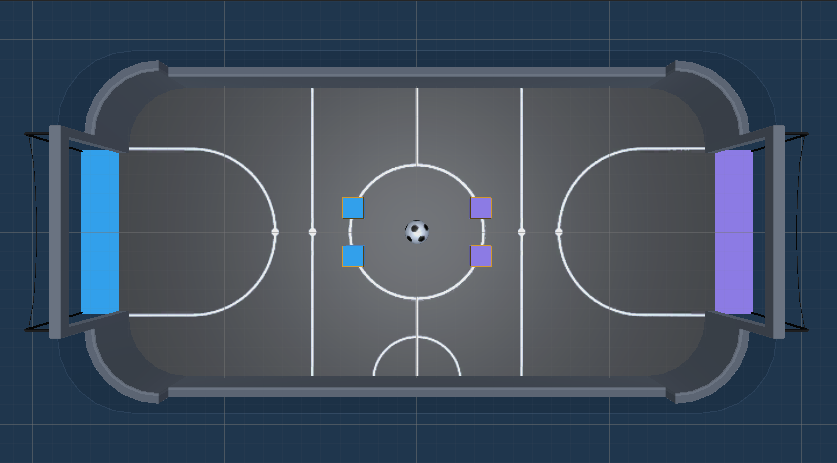
\includegraphics[width=0.7\linewidth]{figures/soccer_field.png}
    \caption{A screenshot of the soccer field taken from the Unity editor}
    \label{fig:soccer_field}
\end{figure}

\noindent
%Overview with image
Here I will lay out the workings of the environment I opted to use, explain the integration with with python, and go over some of the code crucial to its function. This section describes the baseline  modified "Soccer" environment. "Soccer" is the name used in the ML-Agents toolkit. I work with variations on it in \ref{sec:tr:variations}, they all depend on this baseline. The environment I use to train the agent is a simplified version of a game of soccer. 

\subsection{Suitability for my Work}\label{subsec:ip:environment:suitabilty}
At the beginning of this thesis I was faced with the decision whether I should use a preexisting environment or create my own. I opted to make use of an already existing one since this was more in line with my lead question, which asks how an agent is trained. I chose this specific environment because it presents a decent balance between complexity, likelyhood of successful training, intrigue and extensibilty. High extensibilty lowers the barrier to training agents on variations of it, thereby having a measure of how adaptable my methodology it is. Further after the modifications I made to the environment it now also offers continuous control to the agent, this presents an interesting challenge, relevant to real world task, where input is seldom binary.

\subsection{Specifics of Operation}\label{subsec:ip:environment:implementation}
The baseline environment is in function mostly identical to the "Soccer" example environment provided by the Unity ML-Agents toolkit. Here I will go over it's sequence of operation, it's specification, and state all the changes I made to it in order to make it suit my work better. The game of soccer takes place on a bounded field and has four players, distributed across two teams. Each Player is its own Agent, they all act on the same policy and all produce trajectories for it's training. Thereby the policy is trained in play against itself. 

\newpage

\subsubsection{Observations}\label{subsubsec:ip:environment:impl:observations}

\begin{figure}[H]
    \centering
    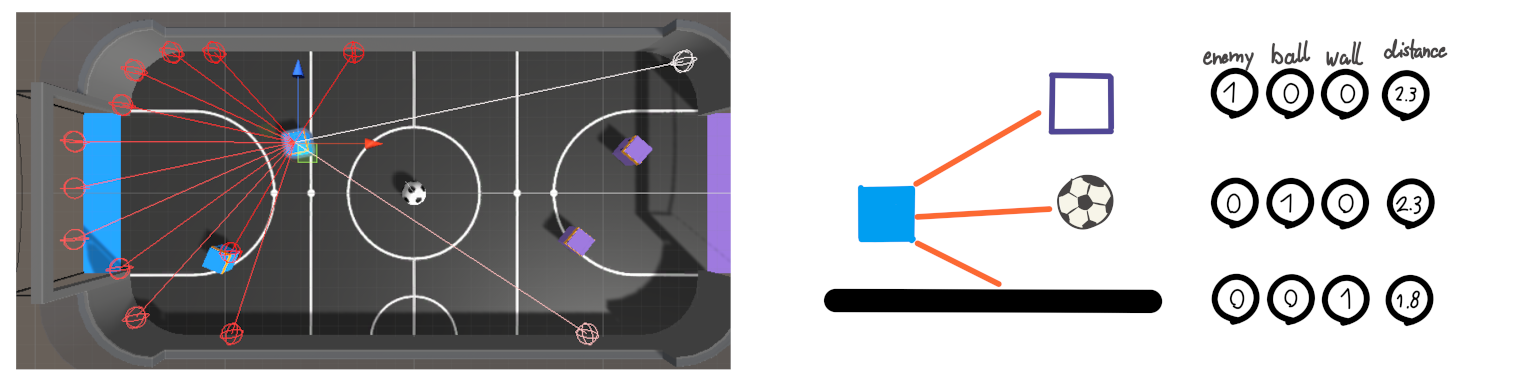
\includegraphics[width=1\linewidth]{figures/ray_sensor.png}
    \caption{Caption}
    \label{fig:ray_sensor}
\end{figure}
\noindent
The "Soccer" example environment uses "Ray Perception Sensors" to create an observation for the agent. A ray perception sensor works by casting a number of rays spread out through a predefined field of view. Along each of these rays a sphere is slid, starting at the agents position and stopping on collision with an object. Each ray contains information about the distance to the object it hit, and its type. The types are predefined, in the case of "Soccer" they are "wall", "enemy", "teammate", "team goal", "enemy goal" and "ball". To the agent a vector is then passed, consisting of the distance to the object the ray struck, as well as its one-hot encoded type. The above figure illustrates how one-hot encoding works and how the observation vectors looks for each ray. The observation vectors are then concatenated to form one single vector, this is then used as the input layer of my policy network. One-hot encoding is commonly used in machine learning where a type information needs to be passed as input, this way separate trainable weights are present for each category. The episode ends if either a goal is score, or a maximum of $600$ time steps pass.

\subsubsection{Episode Start}\label{subsubsec:ip:environment:impl:start}
One subtle but important change I made to the "Soccer" environment is that I randomize agent position and rotation at the beginning of each episode. 

\begin{lstlisting}[basicstyle=\footnotesize]
public override void OnEpisodeBegin() {
    timePenalty = 0;
    m_BallTouch = m_ResetParams.GetWithDefault("ball_touch", 1f);
    transform.rotation = Quaternion.Euler(0, (Convert.ToSingle(random.NextDouble()) - 0.5f) * m_RandomSpawnRotationOffset, 0);
    transform.position = m_Transform + new Vector3((Convert.ToSingle(random.NextDouble()) - 0.5f) * m_RandomSpawnPositionOffset, 0, (Convert.ToSingle(random.NextDouble()) - 0.5f) * m_RandomSpawnPositionOffset);
    agentRb.velocity = Vector3.zero;
    agentRb.angularVelocity = Vector3.zero;
    SetResetParameters();
}
\end{lstlisting}
I made this change because without it during initial testing, agents would come to learn to simply move forward and all clash in to one another. The ball would then fly off in some direction, often scoring a goal for one of the teams. Because of this no real gameplay would arise. While the merits of this change are debatable, i opted for it. This chose was made from personal preference and in the interest gameplay intrigue.

\subsubsection{Actions}\label{subsubsec:ip:environment:impl:actions}
The environment takes continuous action input from the agent. This was not the case in the example environment provided. Three single precision floating point values are expected, they represent forward, lateral, and rotational movement respectively. This is the \code{C\#} code I use to move the agent:

\begin{lstlisting}[basicstyle=\footnotesize]
public void MoveAgent(ActionSegment<float> act) {
    m_KickPower = 0f;

    float longitudinalAxis = Convert.ToSingle(System.Math.Tanh(act[0])) * m_ForwardSpeed;
    float lateralAxis = Convert.ToSingle(System.Math.Tanh(act[1])) * m_LateralSpeed;
    float rotationalAxis = Convert.ToSingle(System.Math.Tanh(act[2]));

    Transform transformTMP;
    (transformTMP = transform).Rotate(transform.up, rotationalAxis * 6.5f);
    agentRb.AddForce(
        (transformTMP.forward * longitudinalAxis +
         transformTMP.right * lateralAxis)
        * m_SoccerSettings.agentRunSpeed,
        ForceMode.VelocityChange);
}
\end{lstlisting}
\noindent
As visible here, I use the scaled arctangent of the action values received. This is to prevent unexpected behaviour which might result when the values the agent selects are too large. The scaling values for forward and lateral speed are the same as the ones used in the "Soccer" example environment. They are \code{m\_LateralSpeed \= 0.3f;} and \code{m\_ForwardSpeed \= 1.0f;}. The \code{agentRunSpeed} is \code{2.0f}.

%Continuous Action Space
%tanh to bind 
\subsubsection{Rewards}\label{subsubsec:ip:environment:impl:rewards}
In the baseline environment I use the rewards provided by the ML-Agents toolkit. The only rewards given to the agent over the course of the episode are on collision with the ball, in which case a reward of \code{0.2} is given, and the end of the episode. This reward is \code{1.0 + timePenalty} if the episode terminated because the agents team managed to score a goal, if the episode ended in a draw or the agent's team lost it is \code{-1.0}. The \code{timePenalty} is accumulated at every time step according to \code{timePenalty -= m_Existential;}, with \code{m_Existential} being the inverse of the maximum episode length. If there was no time penalty it might me more advantageous for the agents to only repeatedly hit the ball instead of scoring goals.
%perform same action for 10 steps
%quit after n steps
%random agent heurisitc 
%Some Code Snippets 
\subsection{Communication with Policy in Python}\label{subsec:ip:environment:communication_python}
One of the reasons the ML-Agents toolkit is particularly appealing is because it allows for extensive control of the environment in Python. The toolkit provides a Python side API with the \code{mlagents} and \code{mlagents_envs} modules. The figure below, taken from \cite[p. 12]{juliani2020unity}, illustrates this interface.

\begin{figure}[H]
    \centering
    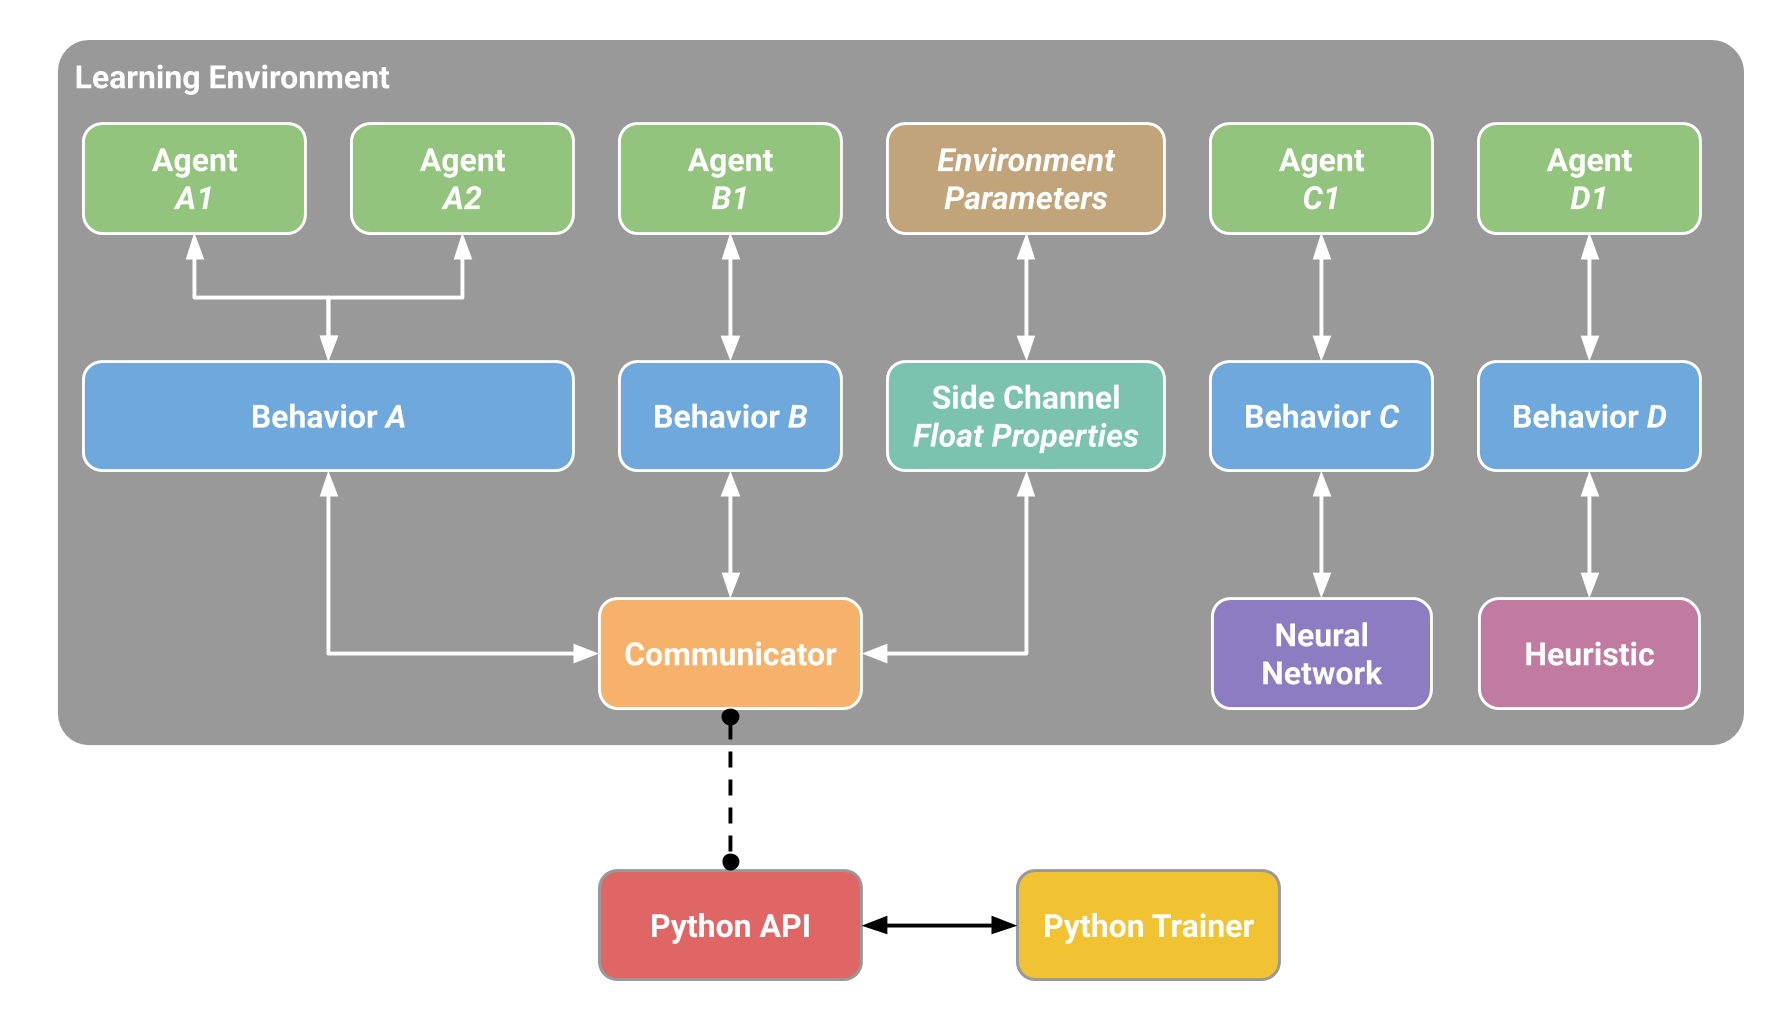
\includegraphics[width=0.75\linewidth]{figures/ml_agents_python_communicator.png}
    \caption{Illustration of communication between Unity and Python}
    \label{fig:python_communicator}
\end{figure}

\noindent
Through the Python API it is possible to train multiple agents, with possibly differing behaviours (formally, each of these behaviours represent a different environment because the observations and actions, as well as the underlying environment functions differ from those of other behaviours, they are effectively different MDPs, see section \ref{sec:MDP}), and even to have yet other agents running on inference (acting on policies which are not being updated, here "Neural Network") or heuristics. This allows for tremendous flexibility not only in training but also enabled me to more fully consider my lead question which also pertains to observation, action and reward design. On the Python side of the ML-Agents training framework there exists, the \code{UnityEnvironment} class. Instantiating it launches, and creates an interface with, a Unity executable \cite[p. 13]{juliani2020unity}. From an instance of \code{UnityEnvironment} information about the observation and action type and size can be obtained. During training and evaluation observations, actions, stepping of the environment, and restarting episodes are all handled through this class's members.

\section{Agent Implementation}\label{sec:ip:agent_implementation}
In this section I will go over the agent implementation in Python. This encompasses the architecture of the Neural Network and the components necessary for training and evaluating an agent.

\subsection{Agent Policy}\label{subsec:ip:agent:network}
In \ref{subsec:ip:environment:implementation} I explained the layout of the observation provided by the environment. With it and knowledge of what type of actions the environment expects, the policy network can be constructed. Both of these can be obtained through an instance of the \code{UnityEnvironment} class, \code{env} in the code below:

\begin{lstlisting}[basicstyle=\footnotesize]
for name, spec in env.behavior_specs.items():
    action_shape = spec.action_shape
    observation_shape = np.sum(np.concatenate(spec.observation_shapes))
\end{lstlisting}

\noindent
I concatenate and sum across \code{spec.observation_shapes} because unity separates ray cast observations up based on internal structure. This separation is useless to me, this is why I undo it here. \code{env.behaviour_specs} is a mapping from behaviour names, to their implementation details. To obtain an action for a continuous environment I sample from a normal distribution following the theory outlined in \ref{subsec:pg:continuous}. For the mean $\mu$ I make use of an MLP \ref{sec:neural_networks}, for the standard deviation $\sigma$ I implement a single trainable parameter for each action. Both are obtained from a Keras model created by by the function found in appendix \ref{appendix:code:network}, following the TensorFlow Keras functional API \cite{noauthor_tensorflow_nodate}\cite{chollet2015keras}. I will first cover the Network used to obtain the mean, then go over how the full normal distribution and action is obtained.

\subsubsection{Neural Network Used for the Mean}\label{subsubsec:ip:agent:policy:mean}
The number of neurons in the last layer before the mean output is the smallest power of two larger than the number of continuous actions and at least $32$. The number of neurons in the input layer is the largest power of two smaller than the dimension of the input vector, and at least four times the number of neurons in the last layer before the output. In between the layers decay in size, each subsequent layer is smaller than the previous by a factor of two. The resulting network looks as follows for the baseline soccer environment:

\begin{figure}[H]
    \centering
    
\includegraphics[width=0.5\linewidth]{figures/placeholder.png}
    \caption{Network Structure}
    \label{fig:network_repr}
\end{figure}

\noindent
This structure provided stable results during initial testing. By creating a comparatively smooth reduction in unit count across layers, each neuron has to encode a limited amount of information. I did not first step up the layer size because for the task at hand, an initial layer size of $256$ seemed sufficient. The last layer does also not have an activation function, and its bias is initialized to be zero. This leads to untrained initial mean values centered on zero. During initial testing this lead to higher stability and likelyhood of convergence on a performant policy. This is also suggested in \citepg{335}. For baseline training I use rectified linear units \cite[pg. 189]{Goodfellow-et-al-2016}, neurons with $\max(0, x)$ as the activation. Neurons using this go by the name of "ReLU", Rectified Linear Units. I initialize the weights in this network using the initialization proposed in \cite[p. 251]{glorot_understanding_2010}, where weights are sampled from $U\left[ -\frac{1}{\sqrt{n}}, \frac{1}{\sqrt{n}} \right]$ with $n$ being the number of units in the previous layer, I will refer to this method of initialization as "glorot uniform". Since I could not find any conclusive evidence on what the best activation and method of initialization are, these choices are mostly arbitrary, and reflect the default options of the Keras API. I cover alternatives in \ref{sec:tr:param_tweaking}.

\subsubsection{Single Trainable Variables for Standard Deviation}\label{subsubsec:ip:agent:policy:std}
Creating input independent trainable variables can be a bit tricky in Keras, especially in conjunction with it's model saving system. However, it is possible by subclassing \code{tensorflow.keras.Layer}. I created such a sub classed custom Keras layer, the respective code follows. In it \code{tensorflow} is aliased by \code{tf}:

\begin{lstlisting}[basicstyle=\footnotesize]
class IndependentTrainableVarLayer(tf.keras.layers.Layer):
    def __init__(self, name: str, initializer: K.initializers.Initializer, shape):
        self.shape = shape
        self.initializer = initializer
        super().__init__()

    def build(self, shape):
        self.x = self.add_weight(name=self.name, shape=self.shape, initializer=self.initializer)

    def call(self, _, **kwargs):
        return tf.identity(self.x)

    def compute_output_shape(self, input_shape):
        return input_shape[0], 1

    def get_config(self):
        return {'shape': self.shape, 'initializer': self.initializer}   
\end{lstlisting}

\noindent
It does not matter what \code{call()} is called on, but Keras expects an input. Further, simply returning self.x is also not possible due to Tensorflows internals. This class is used in the full model code found in \ref{appendix:code:network}.
\subsubsection{Obtaining an Action}
The graph for the combined model for for the mean and standard deviation returned by \ref{appendix:code:network} looks as follows:

\begin{figure}[H]
    \centering
    
\includegraphics[width=0.5\linewidth]{figures/placeholder.png}
    \caption{Structure of baseline Keras model}
    \label{fig:full_model_graph}
\end{figure}

\noindent
From this model the means and standard deviations for a given observation can the be obtained by simply calling it on said observation, an action can then be constructed with \code{tensorflow.random.normal()}. It's first argument is the output shape of the actions, its second are the respective means, and its last the standard deviations. A Keras model expects the first dimension of the input tensor to correspond to a batch of inputs. The resulting output will correspond to the batched input, the model is applied to each item of the input batch. This is convenient since \code{UnityEnvironment} provides the observation for each of its agents in one tensor where the first dimension corresponds to the agents. Thereby the actions for every agent following a particular policy can be obtained with the following method:

\begin{lstlisting}[basicstyle=\footnotesize]
@tf.function
def _get_actions(self, obs) -> tf.Tensor:
    mu, sig = self.policy_network(obs)
    actions: tf.Tensor = tf.random.normal(mu.shape, mu, sig)
    return actions
\end{lstlisting}

\noindent
The \code{@tf.function} decorator results in TensorFlow creating a compilable computational graph in its backend. This enables highly parallel execution. However, in a \code{@tf.function} decorated function, the number of legal operations is limited to the ones supported by TensorFlow. it also returns a \code{tf.Tensor}. For the data contained to be usable for \code{UnityEnvironment}, it needs to be converted to a \code{numpy.ndarray}. This can be done by calling its \code{tf.Tensor.numpy()} method, and caching its return value. 

\subsection{Parameter Update}\label{subsec:ip:agent:training_func}
Having the policy as a Keras model provides for highly efficient training and using Tensorflows inbuilt tools for gradient descent. One of those tools is Tensorflows automatic differentiation. In TensorFlow 2.X this feature is recommended to be accessed through the \code{tensorflow.GradientTape()} context manager. Using it the parameter update presented in \ref{subsec:pg:continuous} can be performed using the following mehtod:

\begin{lstlisting}[basicstyle=\footnotesize]
@tf.function
def _policy_train_step(self, states, actions, returns):
    with tf.GradientTape() as tape:
        mu, sig = self.policy_network(states)
        pdf_value = tf.cast(tf.exp(-0.5 * ((actions - mu) / sig) ** 2), tf.float32) * \(1 / (sig * tf.sqrt(tau)))
        log_probabilities = tf.math.log(pdf_value + 1e-5)
        loss_pi = - returns * log_probabilities
        grads_pi = tape.gradient(loss_pi, self.policy_network.trainable_variables)
    grads_pi = [tf.clip_by_norm(g, self.clip_gradients) for g in grads_pi]
    self.policy_optimizer.apply_gradients(zip(grads_pi, self.policy_network.trainable_variables))
\end{lstlisting}

\noindent
Recall the gradient used in the reinforce update:

\begin{equation*}
    G_t \nabla \ln{\pi(A_t | S_t, \theta_t)}
\end{equation*}

First the mean, here \code{mu}, and the standard deviation of the probability distributions are sampled from the policy network for all observations, here \code{states}. Based on these the probability density can then be obtained for the cached action sampled from the normal distributions during an episode. This corresponds to $\pi(A_t | S_t, \theta_t)$. Next the natural log is applied. Finally, the loss, the expression with respect to which the gradient is derived, is \code{loss_pi}. The returns are computed from the rewards through vectorized operations, the function I use for this is to be found in \ref{appendix:code:returns}. The gradients \code{grads_pi} can be obtained using the alias for the context manager \code{tape}. It is noteworthy that all operations here are element wise. The negative of \code{returns * log_probabilities} is used because gradient ascent, is simply gradient descent performed along the negative gradients. The gradients are clipped to prevent unstable updates when they are overly large. The \code{policy_optimizer} is an implementation of Adam (see \ref{subsec:gd:adam}). This works because for the optimization step only the gradients need to be known. Lastly, in \citepg{328} $\theta$ is updated for every timestep in envery episode sampled from environment interaction. However, since $\nabla J(\theta)$ is the expectation of the gradient above, updating with the average of a batch of samples of this gradient is going to yield a better approximation of $\nabla J(\theta)$, Keras' implementation of Adam does exactly this. 

\subsection{Caching Experience and Batched Training}\label{subsec:ip:agent:archive}
Because of restrictions in the speed in which environment interaction is possible, having only a single agent interact with the environment would quickly become a bottleneck for training time. The base "Soccer" environment provided by unity, is laid out for training $32$ agents simultaneously. This has the consequence that the policy cannot be trained after every episode without throwing out all other trajectories, or changing policy mid episode. To deal with this I use two buffer systems. One, encompassed by the \code{Trajectory} class, stores observations, actions, and rewards of an episode. Once the episode terminates, its returns are computed with the method found in \ref{appendix:code:returns}, and the data is fed to a central dataset. The following preprocessing is then applied to the dataset:

\begin{lstlisting}[basicstyle=\footnotesize]
def train(self, states: tf.Tensor, actions: tf.Tensor, returns: tf.Tensor, measurer: Measurer = None):
    dataset_length = states.shape[0]
    indices = np.arange(dataset_length)
    np.random.shuffle(indices)
    for batch in range(dataset_length // self.batch_size):
        batch_indices = indices[batch * self.batch_size: (batch + 1) * self.batch_size]
        self._policy_train_step(
            tf.gather(states, batch_indices),
            tf.gather(actions, batch_indices),
            tf.gather(returns, batch_indices))
\end{lstlisting}

\noindent
This randomizes the order of the environment interaction samples, and breaks the training process up in to batches. This is not an issue, because the rewards are computed beforehand. The randomization is used to break temporal corelation between samples in a batch, thereby including a broader range of states in it. The rational behind this was that a broader range of states and thereby transitions should lead to a better approximation of $\nabla J(\theta)$. Using Adam each batch correlates to a timestep during optimization. Batch size is one of the parameters explored in \ref{sec:tr:param_tweaking}.

\section{End-to-End Training and Evaluation}\label{sec:ip:training_testing}

\subsection{Code Structure}\label{subsec:ip:tt:class_structure}
Here I will briefly go over the code structure I used. The figure below serves to illustrate it:

\begin{figure}[H]
    \centering
    
\includegraphics[width=0.7\linewidth]{figures/placeholder.png}
    \caption{Code structure used in training}
    \label{fig:code_structure}
\end{figure}

\noindent
The Keras model used for policy approximation is wrapped by a subclass of \code{BasePolicyModel}. As such it implements methods for training based on archived training data, saving the Keras model, and providing actions sampled from the policy. Implementations of \code{Agent} hold this model wrapper, as well as an instance of \code{ BaseTrainingBuffer}, and a dictionary, mapping a \code{Trajectory} to all agents following a conceptual Unity behaviour, which an \code{Agent} corresponds to. The main training loop communicates with \code{Agent} and itself acts as an interface between Unity and the Behaviour specific training code. 


\subsection{The Training Loop}\label{subsec:ip:tt:training_loop}
The code below shows the main loop I use to train agents. This loop generalizes for any number of behaviours, for all of which \code{Agent}s are instantiated dynamically at run time based on parameters. However in the case of the baseline "Soccer" environment, there only is a single behaviour, and thereby agent. \code{agents} is a mapping from Unity's behaviour names to \code{Agent} objects.
\begin{lstlisting}[basicstyle=\footnotesize]
for iteration in range(ParameterData.iterations):
    t_step = 0
    while not all(agent.archive.full for agent in agents.values()):
        for name, agent in agents.items():
            decision_steps, terminal_steps = env.get_steps(name)
            actions = agent.get_actions(np.concatenate(decision_steps.obs, 1))
            env.set_actions(name, actions)
            agent.handle_decision_steps(decision_steps, actions)
            agent.handle_terminal_steps(terminal_steps, ParameterData.discount_factor)
        env.step()
        t_step += 1
        
    for name, agent in agents.items():
        agent.train()
        measures = agent.measurer.finalize_and_collect(name)
        current_time = time.time()
        with writer.as_default():
            for key, value in measures.items():
                if value.shape[0] > 1: tf.summary.histogram(key, value, iteration)
                else: tf.summary.scalar(key, value[0], iteration)
            tf.summary.flush()
        agent.save(ParameterData.model_save_dir + f'{start_time}/{current_time}/')
    env.reset()
\end{lstlisting}
\noindent
The training is performed for a number of iterations preset by a parameter. During each iteration the agents interact with the environment until a sufficient number of samples are accumulated. At each timestep, which here is refering to the synchronized time steps with Unity, decision steps and terminal steps are obtained from Unity. \code{agents} is a mapping from Unity's behaviour names to \code{Agent} objects. \code{decision_steps} is of the type \code{DecisionSteps} and contains the rewards for the previous step, and observations based on which Unity expects actions.
\code{terminal_steps} is of type \code{TerminalSteps} but oposed to decision steps it only contains the rewards for the last timestep in an episode. \code{Agent.handle_decision_steps} and \code{Agent.handle_terminal_steps} both handle training data buffering operations. Once all agents have gathered a sufficient amount of training data, their \code{train()} methods are called and performance as well as stability metrics are collected and logged.

\subsection{Training Variables}\label{subsec:ip:tt:params}
Throughout my work I have introduced many Variables. Below I Provide a short table of the ones used in the baseline environment, where they are used, and their their baseline value. \\
\begin{tabular}{ |p{4cm}||p{3cm}|p{3cm}|p{3cm}|  }
 \hline
 \multicolumn{4}{|c|}{Training Parameters} \\
 \hline
 Parameter & Symbol & Value & Used in Section\\
 \hline
 discount factor & $\gamma$ & 0.99 & \ref{subsec:goals}\\
 samples per iteration &  & $524288 = 2^19$ & \ref{subsec:ip:agent:archive}\\
 batch size &  & $16384 = 2^{14}$ &  \ref{subsec:ip:agent:archive}\\
 learning rate (lr) & $\alpha$ & 0.0003 & \ref{gd:what_is_it}\\
 clipping threshold &  & 10 & \ref{subsec:ip:agent:training_func}\\
 1\textsuperscript{st} momentum decay & $\rho_1$ & 0.9 & \ref{subsec:gd:adam}\\
 2\textsuperscript{nd} momentum decay & $\rho_2$ & 0.999 & \ref{subsec:gd:adam}\\
 activation function &  & ReLU & \ref{subsec:ip:agent:network}\\
 initialization method &  & glorot uniform & \ref{subsec:ip:agent:network}\\
 
 \hline
\end{tabular}

\subsection{Evaluation}\label{subsec:ip:tt:eval} 
To evaluate agent performance during training the metric I use is the average return obtained at each time step. However this brings some limitations when comparing to agents using different parameters because fundamentally, agents are performing self play during training. Since the data of both sides is logged, an increase in agent performance is necessarily also also an increase in it's opponents performance. To account for this I am going to choose parameters based on relative performance. Following the example in \cite{juliani2020unity}, I am going to implement an Elo rating. This is the rating system most famously used in chess. The Elo rating of a player $A$ is updated after a game has been played against $B$ by first calculated the expected score according to:

\begin{equation*}
    E_A = \frac{1}{1+10^{\frac{\left(R_B-R_A\right)}{400}}}
\end{equation*}
\noindent
which can be interpreted as the expected probability of $A$ winning. Then, $A$'s Elo rating $R_A$ can be updated:

\begin{equation*}
    R'_A = R_A + k(S_A-E_A)
\end{equation*}
\noindent
Where $k$ is a constant that determines the weight of each game, in my working i am going to use 4. $S_A$ is the actual score which must also be a valid probability in my case 0 for a loss, 1 for a victory, and 0.5 if the episode terminates because the maximum number of time steps were reached. The number 400 is an arbitrary scaling factor, I follow the example of chess in using it. When evaluating each agent starts out with a score of 1000, then that score is adjusted by playing 1000 games against agents trained on every other permutation of a particular parameter.
\noindent
\\ During training I additionally monitor episode length and the $\mu$ and $\sigma$ values of the normal distribution for continuous actions. This gives me some insight in to training process. In addition to this I log the parameters used in training using TensorBoard, TensorFlow's inbuilt logging system. TensorBoard can host a local server which can the be accessed through a client web GUI:

\begin{figure}[H]
    \centering
    
\includegraphics[width=0.6\linewidth]{figures/placeholder.png}
    \caption{TensorBoard}
    \label{fig:tensorboard}
\end{figure}




% !TEX root = ../maturaarbeit.tex
\chapter{Training the Agent}\label{chap:training}
\section{Baseline Results}\label{sec:tr:baseline_results}
\section{Lower Iteration Times through Parallelization}\label{sec:tr:parallel}
\section{Parameter Tweaking}\label{sec:tr:param_tweaking}
\section{Variations on the Environment}\label{sec:tr:variations}

\chapter{Discussion}\label{chap:discussion}
\section{Validity of Data}\label{sec:disc:significance}
The Error in win percentages between parameters variations is fairly low, games between agents are technically multinomial distributions but because ties are so infrequent (on average $\approx$ 0.5\% of outcomes), and all my data for win probabilities is close to 0.5, i use the "Wade" confidence interval of a binomial\cite[p. 2]{binomial_confidence} to approximate it. I accept a high error level\footnote{$1-\alpha$ can be thought of as the confidence that data falling outside the interval obtained with it, is meaningful.} of $\alpha = 0.2$, as this thesis' focus lies not in perfect parameters, but methods for agent training. The error obtained through this method turns out to be $\approx$0.013\footnote{$p \pm e, e = z\sqrt{p(1-p)/n}$ z is the number of standard deviations within which the percentage of data specified by $\alpha$ falls \cite[p. 2]{binomial_confidence}. It can be obtained by solving $1-\alpha = 2\int_0^z \sqrt{2\pi}^{-1}\exp(-t^2/2)dt$ for $z$.} which corresponds to 1.3\% for all parameters. This corresponds to a difference in elo between parameters of approximately 9\footnote{$\Delta elo = \log_{10}\left(\left(p_{win}^{-1}-1\right)^{-400}\right)$, this increases by $\approx$ 9.0 $\pm$ 0.5 for a percent error of 1 if $p_{win} = 0.5$ $\pm$ 0.12 which all of my data falls in to.} points. The more troublesome error is in the difference between between runs. I cannot control the random seed used for Unity, which makes 1 to 1 repeatability of runs impossible. Monte Carlo approximation of actual parameter performance is prohibitively expensive, instead I estimate the variance in runs as

\begin{equation*}
    \sigma^2 = \frac{1}{n-1} \sum_{i=1}^{n} \left( x_i - \overline{x} \right)^2
\end{equation*}

\noindent
and add to the variance in the binomial confidence interval. The variance of 8 sample runs at 10 million steps is $\approx$ 0.00035, corresponding to an error of $0.028 = 1.3\cdot \sqrt{p(1-p)/2560 + 0.00035}$ if $p_{win} = 0.5 \pm 0.12$, this holds for all my data. however this again imperfect as all data is interdependant. This can be mitigated by letting all sample agent's play against a common opponent, and using the average win percentage of the results for the variance, this methods yields: $\sigma^2 \approx 0.00010$, leading to an error of 0.018, again with $p_{win}$ = 0.5. This is perhaps more representative data as it more accurately reflects the scenario of comparison between parameters, it is the value which I will use, it corresponds to a $\Delta elo$ between parameters of $\approx 13.4$. 
\\Further, 20 million time steps might not be fully representative of agent performance after 100 million. For me, the computational cost of full training runs is simply too high. The elo rating system is a decent indicator of overall performance, but might not give the best parameter choice when testing.

\section{Training Process}
 Agent training for even a relatively simple problem such as this soccer simulation incurs immense computational and temporal cost, including initial testing, though much of this was in parallel, total training time during this thesis including initial testing was roughly 250 hours. Some of this was due to inefficiencies in my methodology, and perhaps poor code performance. As the training algorithm gets more complex and additional variables are introduced, this issue only worsens. 
 \\ Evaluation of training data is also quite difficult, especially in tasks where self play is involved. The elo rating system is a decent indicator of overall performance, but might not give the best parameter choice when testing.
\section{Results}

\section{Outlook}
% !TEX root = ../maturaarbeit.tex
\chapter{Conclusion}\label{chap:conclusion}

% !TEX root = ../maturaarbeit.tex
\printbibliography[
heading=bibintoc,
title={Bibliography}
]

\appendix
\listoffigures 
\listoftables 
% !TEX root = ../maturaarbeit.tex

% !TEX root = ../maturaarbeit.tex

\chapter{Proofs}\label{appendix:proofs}
\section{Policy Gradient Theorem}\label{appendix:sec:pg}
\begin{tcolorbox}[colback=white!5!white,colframe=white!50!black,
  colbacktitle=white!75!black,title=Proof of the Policy Gradient Theorem (episodic case)]
  For the following proof consider $q_\pi(s,a)$ to be defined as $\mathbb{E}_\pi[G_t|S_t=s,A_t=a]$ \citepg{58}, and $\pi$ to be a function of $\theta$.
  \tcblower
  \begin{align*}
  \nabla v_\pi(s) &= \nabla \left[\sum_{a}\pi(a|s)q_\pi(s,a)\right] \MoveEqLeft[1]\\
  &= \sum_{a}\left[\nabla \pi(a|s)q_\pi(s,a)+\pi(a|s)\nabla q_\pi(s,a)\right] \\
  &= \sum \left[\nabla \pi(a|s)q_\pi(s,a) + \pi(a|s)\nabla \sum_{s', r} p(s',r|s,a) (r + v_\pi(s'))\right] \\
  &= \sum \left[\nabla \pi(a|s)q_\pi(s,a) + \pi(a|s) \sum_{s'} p(s'|s,a) v_\pi(s')\right] \\
  &= \sum_{a}\left[\nabla \pi(a|s)q_\pi(a,s) + \pi(a|s)\sum_{s'}p(s'|s,a) \right. \\
  &\qquad \left. \sum_{a'}[\nabla \pi(a'|s')q_\pi(a',s') + \pi(a'|s')\sum_{s''}p(s''|s',a')\nabla v_\pi(s'')]\right] \\
  &= \sum_{x \in \mathset{S}}\sum_{k=0}^{\infty}\operatorname{Pr}(s \rightarrow x, k, \pi)\sum_a \nabla \pi(a|x)q_\pi(x,a), \\
  \intertext{
  after repeated unrolling, where $\operatorname{Pr}(s \rightarrow x, k, \pi)$ is the probability of transitioning from state $s$ to state $x$ in $k$ steps under the policy $\pi$. It is then immediate that 
  } 
  \nabla J(\theta) &= \nabla v_\pi(s_0) \\
  &= \sum_{s}\left(\sum_{k=0}^{\infty} \operatorname{Pr}( s_0 \rightarrow s, k, \pi)\right)\sum_{a}\nabla \pi(a|s)q_\pi(s,a) \\
  &= \sum_s \eta(s) \sum_{a}\nabla \pi(a|s)q_\pi(s,a) \tag*{\citepg{199}} \\
  &= \sum_{s'} \eta(s') \sum_s \frac{\eta(s)}{\sum_{s'}\eta(s')} \sum_{a}\nabla \pi(a|s)q_\pi(s,a) \\
  &= \sum_{s'} \eta(s') \sum_s \mu(s) \sum_{a}\nabla \pi(a|s)q_\pi(s,a) \tag*{\citepg{199}}\\
  &\propto \sum_s \mu(s) \sum_{a}\nabla \pi(a|s)q_\pi(s,a) \tag*{\scshape q.\:e.\:d.}
  \end{align*}
 
\end{tcolorbox}

% !TEX root = ../maturaarbeit.tex

\chapter{Code}\label{appendix:code}
\section{Move Agent Method}\label{appendix:code:move_agent}
\begin{lstlisting}[basicstyle=\footnotesize]
public void MoveAgent(ActionSegment<float> act) {
    m_KickPower = 0f;

    float longitudinalAxis = Convert.ToSingle(System.Math.Tanh(act[0])) * m_ForwardSpeed;
    float lateralAxis = Convert.ToSingle(System.Math.Tanh(act[1])) * m_LateralSpeed;
    float rotationalAxis = Convert.ToSingle(System.Math.Tanh(act[2]));

    Transform transformTMP;
    (transformTMP = transform).Rotate(transform.up, rotationalAxis * 6.5f);
    agentRb.AddForce(
        (transformTMP.forward * longitudinalAxis +
         transformTMP.right * lateralAxis)
        * m_SoccerSettings.agentRunSpeed,
        ForceMode.VelocityChange);
}
\end{lstlisting}

\section{Create Policy Network}\label{appendix:code:network}
\begin{lstlisting}[basicstyle=\footnotesize]
def get_size_decaying_policy_net(
        observation_shape,
        action_shape,
        kernel_initializer: K.initializers.Initializer = K.initializers.HeNormal(seed=0),
        final_continuous_initializer: K.initializers.Initializer = K.initializers.RandomNormal(0, 0.05),
        activation=K.activations.relu,
        bias_mu: float = 0.0,
        bias_sig: float = 0.0,
        sig_single_var: bool = True) -> K.Model:

    node_count = max(int(2 ** np.floor(np.log2(np.sum(observation_shape)))), 64)
    min_node_count = max(int(2 ** np.ceil(np.log2(np.sum(action_shape)))), 32)
    node_count = max(64, min_node_count * 4) if node_count <= min_node_count else node_count

    inputs = K.Input(int(np.sum(observation_shape)))
    dense_layers = [K.layers.Dense(node_count, activation=activation, kernel_initializer=kernel_initializer, name=f'dense_{node_count}')(inputs)]
    node_count /= 2
    layer = 0
    
    while node_count >= min_node_count:
        dense_layers.append(K.layers.Dense(node_count, activation=activation, kernel_initializer=kernel_initializer, name=f'mu_dense_{node_count}')(dense_layers[layer]))
        node_count /= 2
        layer += 1
    mu_out = K.layers.Dense(action_shape, name='mu_out', kernel_initializer=final_continuous_initializer, bias_initializer=K.initializers.constant(bias_mu))(dense_layers[-1])
    
    sig_pre = IndependentTrainableVarLayer('sigpre', K.initializers.constant(bias_sig), action_shape)(inputs)  # it does not matter what this is called on
    sig_out = tf.exp(sig_pre, name='sig_out')  # sigmas in log space so no negative values

    return K.Model(inputs=inputs, outputs=[mu_out, sig_out])

\end{lstlisting}

\section{Compute Returns}\label{appendix:code:returns}
\begin{lstlisting}[basicstyle=\footnotesize]
@staticmethod
def get_fully_discounted_returns(rewards: tf.Tensor, gamma: float):
    horizon = rewards.shape[0]
    gamma = tf.ones([horizon, horizon], tf.float32) * gamma
    exponent = tf.range(horizon, dtype=tf.float32) - tf.expand_dims(tf.range(horizon, dtype=tf.float32), 1)
    mask = tf.pow(gamma, exponent)
    mask = tf.linalg.band_part(mask, 0, -1)  
    returns = rewards * mask
    returns = tf.reduce_sum(returns, axis=1, keepdims=True)
    return returns
\end{lstlisting}

\section{Trajectory Class}\label{appendix:code:trajectory}
\begin{lstlisting}[basicstyle=\footnotesize]
class Trajectory:
    def __init__(self, agent_id, max_len=1000):
        self.max_len = max_len
        self.id = agent_id
        self.states = deque()
        self.actions = deque()
        self.rewards = deque()
        self._out_transitions_states = []
        self._out_transitions_actions = []
        self._out_transitions_returns = []
        self._out_transitions = []
        self._running_idx = 0

    @property
    def full(self):
        return self._running_idx >= self.max_len

    def push(self, state: ndarray, action: ndarray, prev_reward: float): 
        self.states.append(state)
        self.actions.append(action)
        self.rewards.append(prev_reward)

    def finalize(self, final_reward: float, gamma: float):
        diff = self.max_len - self._running_idx
        len_idx = len(self.states) if diff >= len(self.states) else diff
        if self.full:
            raise Exception("trajectory already full, please handle first!!!")
        self.rewards.append(final_reward)
        self._out_transitions_states.append(tf.concat(self.states, 0)[:len_idx])
        self._out_transitions_actions.append(tf.concat(self.actions, 0)[:len_idx])
        self._out_transitions_returns.append(
            self.get_fully_discounted_returns(
                (tf.convert_to_tensor(self.rewards)[1:]), gamma=gamma)[:len_idx])
        self._running_idx += len_idx
        self.flush()

    def pop_transitions(self):
        return (tf.concat(self._out_transitions_states, int(0)),
                tf.concat(self._out_transitions_actions, int(0)),
                tf.concat(self._out_transitions_returns, int(0)))

    def flush(self): 
        self.states.clear()
        self.actions.clear()
        self.rewards.clear()

    def purge(self):
        self.flush()
        self._out_transitions_states.clear()
        self._out_transitions_actions.clear()
        self._out_transitions_returns.clear()
        self._running_idx = 0
\end{lstlisting}
\end{document}